\documentclass[
twoside
% ,openany
,msc
,irfonts
,draft
]{./tex/tehran-thesis}

% در این فایل، دستورها و تنظیمات مورد نیاز، آورده شده است.
%-------------------------------------------------------------------------------------------------------------------
% دستوراتی که پوشه پیش‌فرض زیرفایل‌های tex را مشخص می‌کند.
%\makeatletter
%\def\input@path{{./tex/}}
%\makeatother
% در ورژن جدید زی‌پرشین برای تایپ متن‌های ریاضی، این سه بسته، حتماً باید فراخوانی شود
\usepackage{amsthm,amssymb,amsmath}
\usepackage{MnSymbol}
\usepackage{stmaryrd}
% بسته‌ای برای تنطیم حاشیه‌های بالا، پایین، چپ و راست صفحه
\usepackage[a4paper, top=40mm, bottom=40mm, outer=25mm, inner=35mm]{geometry}
% بسته‌‌ای برای ظاهر شدن شکل‌ها و تعیین آدرس تصاویر
\usepackage[final]{graphicx}
\graphicspath{{./img/}}
% بسته‌های مورد نیاز برای نوشتن کدها، رنگ‌آمیزی آنها و تعیین پوشهٔ کدها
\usepackage[final]{listings}
\usepackage[usenames,dvipsnames,svgnames,table]{xcolor}
\lstset{inputpath=./code/}
% بسته‌ای برای رسم کادر
\usepackage{framed} 
% بسته‌‌ای برای چاپ شدن خودکار تعداد صفحات در صفحه «معرفی پایان‌نامه»
\usepackage{lastpage}
% بسته‌ٔ لازم برای: ۱. تغییر شماره‌گذاری صفحات پیوست. ۲. تصحیح باگ آدرس وب حاوی '%' در مراجع
\usepackage{etoolbox}

%%%%%%%%%%%%%%%%%%%%%%%%%%%%%%%%%%%%
%%% دستورات وابسته به استیل مراجع:
%% اگر از استیل‌های natbib (plainnat-fa، asa-fa، chicago-fa) استفاده می‌کنید، خط زیر را فعال و بعدی‌اش را غیرفعال کنید.
%\usepackage{natbib}
%\newcommand{\citelatin}[1]{\cite{#1}\LTRfootnote{\citeauthor*{#1}}}
%\newcommand{\citeplatin}[1]{\citep{#1}\LTRfootnote{\citeauthor*{#1}}}
%% اگر از سایر استیل‌ها استفاده می‌کنید، خط بالا را غیرفعال و خط‌های زیر را فعال کنید.
\let\citep\cite
\let\citelatin\cite
\let\citeplatin\cite
%%%%%%%%%%%%
% بررسی حالت پیش نویس
\usepackage{ifdraft}
\ifdraft
{%
	% بسته‌ٔ ایجاد لینک‌های رنگی با امکان جهش
	\usepackage[unicode=true,pagebackref=true,
colorlinks,linkcolor=blue,citecolor=blue,final]{hyperref}
	%\usepackage{todonotes}
	\usepackage[firstpage]{draftwatermark}
	\SetWatermarkText{\ \ \ \rl{پیش‌نویس}}
	\SetWatermarkScale{1.2}
}
{ 
	\usepackage[pagebackref=false]{hyperref}
	%\usepackage[disable]{todonotes} % final without TODOs
}

\usepackage[obeyDraft]{todonotes}
\setlength{\marginparwidth}{2cm}

%%%%%%%%%%%%
%%% تصحیح باگ: اگر در مراجع، آدرس وب حاوی '%' بوده و pagebackref فعال باشد، دستورات زیر باید بیایند:
%% برای استیل‌های natbib مثل plainnat-fa، asa-fa، chicago-fa
\makeatletter
\let\ORIG@BR@@lbibitem\BR@@lbibitem
\apptocmd\ORIG@BR@@lbibitem{\endgroup}{}{}
\def\BR@@lbibitem{\begingroup\catcode`\%=12 \ORIG@BR@@lbibitem}
\makeatother
%% برای سایر استیل‌ها
\makeatletter
\let\ORIG@BR@@bibitem\BR@@bibitem
\apptocmd\ORIG@BR@@bibitem{\endgroup}{}{}
\def\BR@@bibitem{\begingroup\catcode`\%=12 \ORIG@BR@@bibitem}
\makeatother
%%%%%%%%%%%%%%%%%%%%%%%%%%%%%%%%%%%%

% بسته‌ لازم برای تنظیم سربرگ‌ها
\usepackage{fancyhdr}
%\usepackage{enumitem}
\usepackage{setspace}
% بسته‌های لازم برای نوشتن الگوریتم
\usepackage{algorithm}
\usepackage{algorithmic}
% بسته‌های لازم برای رسم بهتر جداول
\usepackage{tabulary}
\usepackage{tabularx}
\usepackage{rotating}
% بسته‌های لازم برای رسم تنظیم بهتر شکل‌ها و زیرشکل‌ها
\usepackage[export]{adjustbox}
\usepackage{subfig}
\usepackage[subfigure]{tocloft}
% بسته‌ای برای رسم نمودارها و نیز صفحه مالکیت اثر
\usepackage{tikz}
% بسته‌ای برای ظاهر شدن «مراجع» و «نمایه» در فهرست مطالب
\usepackage[nottoc]{tocbibind}
% دستورات مربوط به ایجاد نمایه
\usepackage{makeidx}
\makeindex
%%% بسته ایجاد واژه‌نامه با xindy
\usepackage[xindy,toc,acronym,nonumberlist=true]{glossaries}

% بسته‌ای برای افزودن تورفتگی به ابتدای اولین پاراگراف هر بخش
\usepackage{indentfirst}

% بسته زیر باگ ناشی از فراخوانی بسته‌های زیاد را برطرف می‌کند.
\usepackage{morewrites}
%%%%%%%%%%%%%%%%%%%%%%%%%%
% فراخوانی بسته زی‌پرشین (باید آخرین بسته باشد)
\usepackage[extrafootnotefeatures,  displaymathdigits=default]{xepersian}

\usepackage{import}

\makeatletter
% تعریف قلم فارسی و انگلیسی و مکان قلم‌ها
\if@irfonts
\settextfont[Path={./font/}, BoldFont={IRLotusICEE_Bold.ttf}, BoldItalicFont={IRLotusICEE_BoldIranic.ttf}, ItalicFont={IRLotusICEE_Iranic.ttf},Scale=1.2]{IRLotusICEE.ttf}
% LiberationSerif or FreeSerif as free equivalents of Times New Roman
\setlatintextfont[Path={./font/}, BoldFont={LiberationSerif-Bold.ttf}, BoldItalicFont={LiberationSerif-BoldItalic.ttf}, ItalicFont={LiberationSerif-Italic.ttf},Scale=1]{LiberationSerif-Regular.ttf}
% چنانچه می‌خواهید اعداد در فرمول‌ها، انگلیسی باشد، خط زیر را غیرفعال کنید
% و گزینهٔ displaymathdigits=persian را از خط ۱۰۹ حذف کنید.
\setdigitfont[Path={./font/}, Scale=1.2]{IRLotusICEE.ttf}
% تعریف قلم‌های فارسی و انگلیسی اضافی برای استفاده در بعضی از قسمت‌های متن
\setiranicfont[Path={./font/}, Scale=1.3]{IRLotusICEE_Iranic.ttf}				% ایرانیک، خوابیده به چپ
\setmathsfdigitfont[Path={./font/}]{IRTitr.ttf}
\defpersianfont\titlefont[Path={./font/}, Scale=1]{IRTitr.ttf}
% برای تعریف یک قلم خاص عنوان لاتین، خط بعد را فعال و ویرایش کنید و خط بعد از آن را غیرفعال کنید.
% \deflatinfont\latintitlefont[Scale=1]{LiberationSerif}
\font\latintitlefont=cmssbx10 scaled 2300 %cmssbx10 scaled 2300
\else
\settextfont{XB Niloofar}
\setlatintextfont{Junicode}
% چنانچه می‌خواهید اعداد در فرمول‌ها، انگلیسی باشد، خط زیر را غیرفعال کنید
% و گزینهٔ displaymathdigits=persian را از خط ۱۰۹ حذف کنید.
\setdigitfont{XB Niloofar}
% تعریف قلم‌های فارسی و انگلیسی اضافی برای استفاده در بعضی از قسمت‌های متن
% \setmathsfdigitfont{XB Titre}
\defpersianfont\titlefont{XB Titre}
\deflatinfont\latintitlefont[Scale=1.1]{Junicode}
\fi
\makeatother

% برای استفاده از قلم نستعلیق خط بعد را فعال کنید.
% \defpersianfont\nastaliq[Scale=1.2]{IranNastaliq}


%%%%%%%%%%%%%%%%%%%%%%%%%%
% راستچین شدن todonotes
\presetkeys{todonotes}{align=right,textdirection=righttoleft}{}
\makeatletter
\providecommand\@dotsep{5}
\def\listtodoname{فهرست کارهای باقیمانده}
\def\listoftodos{\noindent{\Large\vspace{10mm}\textbf{\listtodoname}}\@starttoc{tdo}}
\renewcommand{\@todonotes@MissingFigureText}{شکل}
\renewcommand{\@todonotes@MissingFigureUp}{شکل}
\renewcommand{\@todonotes@MissingFigureDown}{جاافتاده}
\makeatother
% دستوری برای حذف کلمه «چکیده»
% \renewcommand{\abstractname}{}
% دستوری برای حذف کلمه «abstract»
%\renewcommand{\latinabstract}{}
% دستوری برای تغییر نام کلمه «اثبات» به «برهان»
\renewcommand\proofname{\textbf{برهان}}
% دستوری برای تغییر نام کلمه «کتاب‌نامه» به «مراجع»
\renewcommand{\bibname}{مراجع}
% دستوری برای تعریف واژه‌نامه انگلیسی به فارسی
\newcommand\persiangloss[2]{#1\dotfill\lr{#2}\\}
% دستوری برای تعریف واژه‌نامه فارسی به انگلیسی 
\newcommand\englishgloss[2]{#2\dotfill\lr{#1}\\}
% تعریف دستور جدید «\پ» برای خلاصه‌نویسی جهت نوشتن عبارت «پروژه/پایان‌نامه/رساله»
\newcommand{\پ}{پروژه/پایان‌نامه/رساله }

%\newcommand\BackSlash{\char`\\}

%%%%%%%%%%%%%%%%%%%%%%%%%%
% \SepMark{-}

% تعریف و نحوه ظاهر شدن عنوان قضیه‌ها، تعریف‌ها، مثال‌ها و ...
\theoremstyle{definition}
\newtheorem{definition}{تعریف}[section]
\theoremstyle{theorem}
\newtheorem{theorem}[definition]{قضیه}
\newtheorem{lemma}[definition]{لم}
\newtheorem{proposition}[definition]{گزاره}
\newtheorem{corollary}[definition]{نتیجه}
\newtheorem{remark}[definition]{ملاحظه}
\theoremstyle{definition}
\newtheorem{example}[definition]{مثال}

%\renewcommand{\theequation}{\thechapter-\arabic{equation}}
%\def\bibname{مراجع}
\numberwithin{algorithm}{chapter}
\def\listalgorithmname{فهرست الگوریتم‌ها}
\def\listfigurename{فهرست تصاویر}
\def\listtablename{فهرست جداول}

% دستور های لازم برای تعریف ترجمهٔ دستورات الگوریتم
\makeatletter
\renewcommand{\algorithmicrequire}{\if@RTL\textbf{ورودی:}\else\textbf{Require:}\fi}
\renewcommand{\algorithmicensure}{\if@RTL\textbf{خروجی:}\else\textbf{Ensure:}\fi}
\renewcommand{\algorithmicend}{\if@RTL\textbf{پایان}\else\textbf{end}\fi}
\renewcommand{\algorithmicif}{\if@RTL\textbf{اگر}\else\textbf{if}\fi}
\renewcommand{\algorithmicthen}{\if@RTL\textbf{آنگاه}\else\textbf{then}\fi}
\renewcommand{\algorithmicelse}{\if@RTL\textbf{وگرنه}\else\textbf{else}\fi}
\renewcommand{\algorithmicfor}{\if@RTL\textbf{برای}\else\textbf{for}\fi}
\renewcommand{\algorithmicforall}{\if@RTL\textbf{برای هر}\else\textbf{for all}\fi}
\renewcommand{\algorithmicdo}{\if@RTL\textbf{انجام بده}\else\textbf{do}\fi}
\renewcommand{\algorithmicwhile}{\if@RTL\textbf{تا زمانی که}\else\textbf{while}\fi}
\renewcommand{\algorithmicloop}{\if@RTL\textbf{تکرار کن}\else\textbf{loop}\fi}
\renewcommand{\algorithmicrepeat}{\if@RTL\textbf{تکرار کن}\else\textbf{repeat}\fi}
\renewcommand{\algorithmicuntil}{\if@RTL\textbf{تا زمانی که}\else\textbf{until}\fi}
\renewcommand{\algorithmicprint}{\if@RTL\textbf{چاپ کن}\else\textbf{print}\fi}
\renewcommand{\algorithmicreturn}{\if@RTL\textbf{بازگردان}\else\textbf{return}\fi}
\renewcommand{\algorithmicand}{\if@RTL\textbf{و}\else\textbf{and}\fi}
\renewcommand{\algorithmicor}{\if@RTL\textbf{و یا}\else\textbf{or}\fi} % TODO add better translate
\renewcommand{\algorithmicxor}{\if@RTL\textbf{یا}\else\textbf{xor}\fi} % TODO add better translate
\renewcommand{\algorithmicnot}{\if@RTL\textbf{نقیض}\else\textbf{not}\fi}
\renewcommand{\algorithmicto}{\if@RTL\textbf{تا}\else\textbf{to}\fi}
\renewcommand{\algorithmicinputs}{\if@RTL\textbf{ورودی‌ها}\else\textbf{inputs}\fi}
\renewcommand{\algorithmicoutputs}{\if@RTL\textbf{خروجی‌ها}\else\textbf{outputs}\fi}
\renewcommand{\algorithmicglobals}{\if@RTL\textbf{متغیرهای عمومی}\else\textbf{globals}\fi}
\renewcommand{\algorithmicbody}{\if@RTL\textbf{انجام بده}\else\textbf{do}\fi}
\renewcommand{\algorithmictrue}{\if@RTL\textbf{درست}\else\textbf{true}\fi}
\renewcommand{\algorithmicfalse}{\if@RTL\textbf{نادرست}\else\textbf{false}\fi}
\renewcommand{\algorithmicendif}{\algorithmicend\textbf{ شرط }\algorithmicif}
\renewcommand{\algorithmicendfor}{\algorithmicend\textbf{ حلقهٔ }\algorithmicfor}
\renewcommand{\algorithmicendwhile}{\algorithmicend\textbf{ حلقهٔ }\algorithmicwhile}
\renewcommand{\algorithmicendloop}{\algorithmicend\textbf{ حلقهٔ }\algorithmicloop}
\renewcommand{\algorithmiccomment}[1]{\{{\itshape #1}\}}
\makeatletter

%%%%%%%%%%%%%%%%%%%%%%%%%%%%
%%% دستورهایی برای سفارشی کردن سربرگ صفحات:
%\newcommand{\SetHeader}[1]{
% دستور زیر معادل با گزینه twoside است.
%\csname@twosidetrue\endcsname
\pagestyle{fancy}
%% دستورات زیر سبک صفحات fancy را تغییر می‌دهد:
% O=Odd, E=Even, L=Left, R=Right
% در صورت oneside بودن، عنوان فصل، سمت چپ ظاهر می‌شود.
\fancyhead{}
\fancyhead[OL]{\small\leftmark}
\fancyhead[ER]{\small\leftmark}
\fancyhead[OR]{\footnotesize\rightmark}
\fancyhead[EL]{\footnotesize\rightmark}
\renewcommand{\headrulewidth}{0.75pt}
% شکل‌دهی شماره و عنوان فصل در سربرگ
\renewcommand{\chaptermark}[1]{\markboth{فصل~\thechapter:\ #1}{}}
\makeatletter
\renewcommand{\rightmark}[1]{\@title}
\makeatother
%}
%%%%%%%%%%%%%%%%%%%%%%%%%%%%
%\def\MATtextbaseline{1.5}
%\renewcommand{\baselinestretch}{\MATtextbaseline}
\doublespacing
%%%%%%%%%%%%%%%%%%%%%%%%%%%%%
% دستوراتی برای اضافه کردن کلمه «فصل» در فهرست مطالب

\newlength\mylenprt
\newlength\mylenchp
\newlength\mylenapp

\renewcommand\cftpartpresnum{\partname~}
\renewcommand\cftchappresnum{\chaptername~}
\renewcommand\cftchapaftersnum{:}

\settowidth\mylenprt{\cftpartfont\cftpartpresnum\cftpartaftersnum}
\settowidth\mylenchp{\cftchapfont\cftchappresnum\cftchapaftersnum}
\settowidth\mylenapp{\cftchapfont\appendixname~\cftchapaftersnum}
\addtolength\mylenprt{\cftpartnumwidth}
\addtolength\mylenchp{\cftchapnumwidth}
\addtolength\mylenapp{\cftchapnumwidth}

\setlength\cftpartnumwidth{\mylenprt}
\setlength\cftchapnumwidth{\mylenchp}	

\makeatletter
{\def\thebibliography#1{\chapter*{\refname\@mkboth
   {\uppercase{\refname}}{\uppercase{\refname}}}\list
   {[\arabic{enumi}]}{\settowidth\labelwidth{[#1]}
   \rightmargin\labelwidth
   \advance\rightmargin\labelsep
   \advance\rightmargin\bibindent
   \itemindent -\bibindent

   \listparindent \itemindent
   \parsep \z@
   \usecounter{enumi}}
   \def\newblock{}
   \sloppy
   \sfcode`\.=1000\relax}}
   
%اگر مایلید در شماره گذاری حرفی و ابجد به جای آ از الف استفاده شود دستورات زیر را فعال کنید.   
%\def\@Abjad#1{%
%  \ifcase#1\or الف\or ب\or ج\or د%
%           \or هـ\or و\or ز\or ح\or ط%
%           \or ی\or ک\or ل\or م\or ن%
%           \or س\or ع\or ف\or ص%
%           \or ق\or ر\or ش\or ت\or ث%
%            \or خ\or ذ\or ض\or ظ\or غ%
%            \else\@ctrerr\fi}
%
% \def\abj@num@i#1{%
%   \ifcase#1\or الف\or ب\or ج\or د%
%            \or هـ‍\or و\or ز\or ح\or ط\fi

%   \ifnum#1=\z@\abjad@zero\fi}   
%  
%   \def\@harfi#1{\ifcase#1\or الف\or ب\or پ\or ت\or ث\or

% ج\or چ\or ح\or خ\or د\or ذ\or ر\or ز\or ژ\or س\or ش\or ص\or ض\or ط\or ظ\or ع\or غ\or

% ف\or ق\or ک\or گ\or ل\or م\or ن\or و\or ه\or ی\else\@ctrerr\fi}

%
\makeatother

%%% امکان درج کد در سند
% در این قسمت رنگ، قلم و قالب‌بندی قسمت‌های مختلف یک کد تعیین می‌شود. 
\lstdefinestyle{myStyle}{
	basicstyle=\ttfamily, % whole listing /w verbatim font
	keywordstyle=\color{blue}\bfseries, % bold black keywords
	identifierstyle=, % nothing happens
	commentstyle=\color{LimeGreen}, % green comments
	stringstyle=\ttfamily\color{red}, % red typewriter font for strings
	showstringspaces=false % no special string spaces
	breaklines=true,
	breakatwhitespace=false,
	numbers=right, % line number formats
	numberstyle=\footnotesize\lr,
	numbersep=-10pt,
	frame=single,
	captionpos=b,
	captiondirection=RTL
}
\lstset{style=myStyle} % command to set default style
\def\lstlistingname{\rl{برنامهٔ}}
\def\lstlistlistingname{\rl{فهرست برنامه‌ها}}


% for numbering subsubsections
\setcounter{secnumdepth}{3}
%to include subsubsections in the table of contents
\setcounter{tocdepth}{3}

\makeatletter
\renewcommand{\p@subfigure}{\thefigure.}
\makeatother


\newcommand{\s}[1]{\{#1\}}
\newcommand{\sem}[1]{\llbracket #1 \rrbracket}
\newcommand{\his}[1]{\langle #1 \rangle}
\newcommand{\e}{\emptyset}
\newcommand{\la}{\leftarrow}
\newcommand{\ra}{\rightarrow}
\newcommand{\teq}{\triangleq}
\newcommand{\crd}[4][above]{
    \node[draw,circle,inner sep=2pt,fill,label={[#1]:#4}] at (#2,#3) {};
}


% !TeX root=../main.tex
\university{دانشگاه تهران}
\college{پردیس دانشکده‌های فنی}
\faculty{دانشکده مهندسی برق و کامپیوتر}
\department{}
\subject{مهندسی کامپیوتر}
\field{نرم‌افزار}
\title{توضیح خطا در شبکه‌های مبتنی بر نرم‌افزار با استفاده از استدلال مبتنی بر علیت}
\firstsupervisor{دکتر حسین حجت}
\firstsupervisorrank{استادیار}
% \secondsupervisor{دکتر محمدرضا موسوی}
% \secondsupervisorrank{استادیار}
\firstadvisor{دکتر محمدرضا موسوی}
\firstadvisorrank{استاد}
\internaljudge{}
\internaljudgerank{}
\externaljudge{}
\externaljudgerank{}
\externaljudgeuniversity{}
% نام نماینده کمیته تحصیلات تکمیلی در دانشکده \ گروه
\graduatedeputy{}
\graduatedeputyrank{}
% نام دانشجو را وارد کنید
\name{امیرحسین}
% نام خانوادگی دانشجو را وارد کنید
\surname{صیحانی}
% شماره دانشجویی دانشجو را وارد کنید
\studentID{810198198}
% تاریخ پایان‌نامه را وارد کنید
\thesisdate{شهریور ۱۴۰۱}
%\projectLabel{پایان‌نامه}

%\degree{}
%%%%%%%%%%%%%%%%%%%%%%%%%%%%%%%%%%%%%%%%%%%%%%%%%%%%
%% پایان‌نامه خود را تقدیم کنید! %%
\dedication
{
{\Large تقدیم به:}\\
\begin{flushleft}{
	\huge
	همسر و فرزندانم\\
	\vspace{7mm}
	و\\
	\vspace{7mm}
	پدر و مادرم
}
\end{flushleft}
}
\fa-abstract{
	جایگزینی شبکه‌های کامپیوتری سنتی با شبکه‌ها مبتنی بر نرم‌افزار%
\lf{Software-Defined Network}
باعث شده است تا استفاده از روش‌ها و ابزار‌های مبتنی بر روش‌های صوری%
\lf{Formal Methods}
برای درستی‌سنجی%
\lf{Verification}
این شبکه‌ها تسهیل شود.
با اینکه درستی‌سنجی لازمه‌ی رفع‌ایراد در سیستم‌ها است، اما پس از مشخص شدن وجود خطا در سیستم، پیدا کردن دلیل این مساله که چرا سیستم دچار خطا شده است همچنان بر عهده‌ی کاربر است و لازم است که او با تحلیل و بررسی سیستم علت مشکل را پیدا کند و ایراد سیستم را بر طرف کند.
ابزار‌های درستی‌سنجی در صورتی که سیستم مطابق انتظار رفتار نکند یک مثال‌نقض یا گواهی برای اثبات این موضوع به کاربر ارائه می‌کنند اما این مدارک به تنهایی و بدون پردازش بیشتر اطلاعات کافی از چرایی مشکل در اختیار نمی‌گذارند.

توضیح پدیده‌ها در متون فلسفه قرن‌ها مورد مطالعه قرار گرفته است و نتایج این مطالعات در قالب اصول استدلال مبتنی بر خلاف واقع%
\lf{Counterfactual Reasoning}
تجمیع شده است.
هالپرن%
\lf{Joseph Y. Halpern}
و پرل%
\lf{Judea Pearl}
یک فرمولاسیون ریاضی برای پیدا کردن علت واقعی%
\lf{Actual Cause}
بر اساس استدلال مبتنی بر خلاف واقع ارائه کرده‌اند که در پژوهش‌های متعددی برای ارائه توضیح در مورد خطای رخ داده در سیستم و پیدا کردن علت واقعی آن مورد استفاده قرار گرفته است.

در این پژوهش از مفهوم علت واقعی ارائه شده توسط هالپرن و پرل برای توضیح خطا در شبکه‌های مبتنی بر نرم‌افزار استفاده می‌شود.
به صورت دقیق‌تر در این پژوهش یک مدل علّی%
\lf{Casual Model}
ارائه می‌شود که با استفاده از آن می‌توان در مورد ساختارهای شبکه، مانند وجود هم‌روندی یا ترتیب میان به‌روز رسانی‌های شبکه، برای پیدا کردن علت واقعی رفتار نا امن شبکه استدلال کرد.

در این پژوهش برای توصیف نرم‌افزار شبکه از زبان نت‌کت‌ پویا%
\lf{DyNetKAT}
استفاده می‌شود.
نت‌کت پویا یک سطح‌ بالا برنامه‌ نویسی شبکه است که بر پایه نت‌کت%
\lf{NetKAT}
 بنا شده و با وجود اینکه مینیمال بودن آن را حفظ کرده امکان توصیف به‌روز رسانی‌های پویای شبکه را فراهم می‌کند.
در این پژوهش از ساختمان رویداد%
\lf{Event Structure}
به عنوان مدل معنایی%
\lf{Semantic Model}
برنامه‌های نت‌کت پویا استفاده می‌شود.
ساختمان رویداد امکان توصیف صریح هم‌روندی را فراهم می‌کند که این موضوع سبب می‌شود چنین روابطی میان پردازه‌ها را هم بتوان به عنوان علت خطا در نظر گرفت، امری که با استفاده از مدل‌های برگ‌برگ شده%
\lf{Interleaving}
امکان پذیر نیست.
روش ارائه شده در این پژوهش برای پیدا کردن علت نقض چند ویژگی مطرح 
شبکه، مثلا نبود دور، مورد استفاده قرار گرفته است و بررسی این مساله‌ها نشان می‌دهد که علت‌های پیدا شده با شهود موجود از علت خطا در سیستم تطابق دارند.

}
\keywords{استدلال مبتنی بر علیت، ساختمان رویداد، درستی‌سنجی،
 شبکه‌های مبتنی بر نرم‌افزار}

% !TeX root=../main.tex
% در این فایل، عنوان پایان‌نامه، مشخصات خود و چکیده پایان‌نامه را به انگلیسی، وارد کنید.

%%%%%%%%%%%%%%%%%%%%%%%%%%%%%%%%%%%%
\latinuniversity{University of Tehran}
\latincollege{College of Engineering}
\latinfaculty{Faculty of Electrical and Computer Engineering}
\latindepartment{}
\latinsubject{Computer Engineering}
\latinfield{Software Engineering}
\latintitle{Explaining Software-Defined Networks Failures using Causal Reasoning}
\firstlatinsupervisor{Dr. Hossein Hojjat}
\secondlatinsupervisor{Dr. Mohammad Reza Mousavi}
\firstlatinadvisor{First Advisor}
%\secondlatinadvisor{Second Advisor}
\latinname{Amir Hossein}
\latinsurname{Seyhani}
\latinthesisdate{September 2022}
\latinkeywords{Writing Thesis, Template, \LaTeX, \XePersian}
\en-abstract{
This thesis studies on writing projects, theses and dissertations using tehran-thesis class. It ...
}

%%% تنظیمات مربوط به بسته  glossaries
%%% تعریف استایل برای واژه‌نامه فارسی به انگلیسی، در این استایل واژه‌های فارسی در سمت راست و واژه‌های انگلیسی در سمت چپ خواهند آمد. از حالت گروه ‌بندی استفاده می‌کنیم، 
%%% یعنی واژه‌ها در گروه‌هایی به ترتیب حروف الفبا مرتب می‌شوند، مثلا:
%%% الف
%%% افتصاد ................................... Economy
%%% اشکال ........................................ Failure
%%% ش
%%% شبکه ...................................... Network
\newglossarystyle{myFaToEn}{%
	\renewenvironment{theglossary}{}{}
	\renewcommand*{\glsgroupskip}{\vskip 10mm}
	\renewcommand*{\glsgroupheading}[1]{\subsection*{\glsgetgrouptitle{##1}}}
	\renewcommand*{\glossentry}[2]{\noindent\glsentryname{##1}\dotfill\space \glsentrytext{##1}
		
	}
}

%% % تعریف استایل برای واژه‌نامه انگلیسی به فارسی، در این استایل واژه‌های فارسی در سمت راست و واژه‌های انگلیسی در سمت چپ خواهند آمد. از حالت گروه ‌بندی استفاده می‌کنیم، 
%% % یعنی واژه‌ها در گروه‌هایی به ترتیب حروف الفبا مرتب می‌شوند، مثلا:
%% % E
%%% Economy ............................... اقتصاد
%% % F
%% % Failure................................... اشکال
%% %N
%% % Network ................................. شبکه

\newglossarystyle{myEntoFa}{%
	%%% این دستور در حقیقت عملیات گروه‌بندی را انجام می‌دهد. بدین صورت که واژه‌ها در بخش‌های جداگانه گروه‌بندی می‌شوند، 
	%%% عنوان بخش همان نام حرفی است که هر واژه در آن گروه با آن شروع شده است. 
	\renewenvironment{theglossary}{}{}
	\renewcommand*{\glsgroupskip}{\vskip 10mm}
	\renewcommand*{\glsgroupheading}[1]{\begin{LTR} \subsection*{\glsgetgrouptitle{##1}} \end{LTR}}
	%%% در این دستور نحوه نمایش واژه‌ها می‌آید. در این جا واژه فارسی در سمت راست و واژه انگلیسی در سمت چپ قرار داده شده است، و بین آن با نقطه پر می‌شود. 
	\renewcommand*{\glossentry}[2]{\noindent\glsentrytext{##1}\dotfill\space \glsentryname{##1}
		
	}
}

%%% تعیین استایل برای فهرست اختصارات
\newglossarystyle{myAbbrlist}{%
	%%% این دستور در حقیقت عملیات گروه‌بندی را انجام می‌دهد. بدین صورت که اختصارات‌ در بخش‌های جداگانه گروه‌بندی می‌شوند، 
	%%% عنوان بخش همان نام حرفی است که هر اختصار در آن گروه با آن شروع شده است. 
	\renewenvironment{theglossary}{}{}
	\renewcommand*{\glsgroupskip}{\vskip 10mm}
	\renewcommand*{\glsgroupheading}[1]{\begin{LTR} \subsection*{\glsgetgrouptitle{##1}} \end{LTR}}
	%%% در این دستور نحوه نمایش اختصارات می‌آید. در این جا حالت کوچک اختصار در سمت چپ و حالت بزرگ در سمت راست قرار داده شده است، و بین آن با نقطه پر می‌شود. 
	\renewcommand*{\glossentry}[2]{\noindent\Glsentrylong{##1}\dotfill\space \glsentrytext{##1} 
		
	}
	%%% تغییر نام محیط abbreviation به فهرست اختصارات
	\renewcommand*{\acronymname}{\rl{فهرست اختصارات}}
}

%%% برای اجرا xindy بر روی فایل .tex و تولید واژه‌نامه‌ها و فهرست اختصارات و فهرست نمادها یکسری  فایل تعریف شده است.‌ Latex داده های مربوط به واژه‌نامه و .. را در این 
%%%  فایل‌ها نگهداری می‌کند. مهم‌ترین option‌ این قسمت این است که 
%%% عنوان واژه‌نامه‌ها و یا فهرست اختصارات و یا فهرست نمادها را می‌توانید در این‌جا مشخص کنید. 
%%% در این جا عباراتی مثل glg، gls، glo و ... پسوند فایل‌هایی است که برای xindy بکار می‌روند. 
\newglossary[glg]{english}{gls}{glo}{واژه‌نامهٔ انگلیسی به فارسی}
\newglossary[blg]{persian}{bls}{blo}{واژه‌نامهٔ فارسی به انگلیسی}
\makeglossaries
\glsdisablehyper
%%% تعاریف مربوط به تولید واژه‌نامه و فهرست اختصارات و فهرست نمادها
%%%  در این فایل یکسری دستورات عمومی برای وارد کردن واژه‌نامه آمده است.
%%%  به دلیل این‌که قرار است این دستورات پایه‌ای را بازنویسی کنیم در این‌جا تعریف می‌کنیم. 
\let\oldgls\gls
\let\oldglspl\glspl

\makeatletter

\renewrobustcmd*{\gls}{\@ifstar\@msgls\@mgls}
\newcommand*{\@mgls}[1] {\ifthenelse{\equal{\glsentrytype{#1}}{english}}{\oldgls{#1}\glsuseri{f-#1}}{\lr{\oldgls{#1}}}}
\newcommand*{\@msgls}[1]{\ifthenelse{\equal{\glsentrytype{#1}}{english}}{\glstext{#1}\glsuseri{f-#1}}{\lr{\glsentryname{#1}}}}

\renewrobustcmd*{\glspl}{\@ifstar\@msglspl\@mglspl}
\newcommand*{\@mglspl}[1] {\ifthenelse{\equal{\glsentrytype{#1}}{english}}{\oldglspl{#1}\glsuseri{f-#1}}{\oldglspl{#1}}}
\newcommand*{\@msglspl}[1]{\ifthenelse{\equal{\glsentrytype{#1}}{english}}{\glsplural{#1}\glsuseri{f-#1}}{\glsentryplural{#1}}}

\makeatother

\newcommand{\newword}[4]{
	\newglossaryentry{#1}     {type={english},name={\lr{#2}},plural={#4},text={#3},description={}}
	\newglossaryentry{f-#1} {type={persian},name={#3},text={\lr{#2}},description={}}
}

%%% بر طبق این دستور، در اولین باری که واژه مورد نظر از واژه‌نامه وارد شود، پاورقی زده می‌شود. 
\defglsentryfmt[english]{\glsgenentryfmt\ifglsused{\glslabel}{}{\LTRfootnote{\glsentryname{\glslabel}}}}

%%% بر طبق این دستور، در اولین باری که واژه مورد نظر از فهرست اختصارات وارد شود، پاورقی زده می‌شود. 
\defglsentryfmt[acronym]{\glsentryname{\glslabel}\ifglsused{\glslabel}{}{\footnote{\glsentrydesc{\glslabel}}}}


%%%%%% ============================================================================================================

%%============================ دستور برای قرار دادن فهرست اختصارات 
\newcommand{\printabbreviation}{
	%\cleardoublepage
	%\phantomsection
	\baselineskip=.75cm
	\setglossarystyle{myAbbrlist}
	%\begin{LTR}
		\Oldprintglossary[type=acronym]	
	%\end{LTR}
	\clearpage
}%

\newcommand{\printacronyms}{\printabbreviation}
%%% در این جا محیط هر دو واژه‌نامه را باز تعریف کرده ایم، تا اولا مشکل قرار دادن صفحه اضافی را حل کنیم، ثانیا عنوان واژه‌نامه ها را با دستور addcontentlist وارد فهرست مطالب کرده ایم.
\let\Oldprintglossary\printglossary
\renewcommand{\printglossary}{
	\let\appendix\relax
	%% تنظیم کننده فاصله بین خطوط در این قسمت
	\clearpage
	%\phantomsection
	%% این دستور موجب این می‌شود که واژه‌نامه‌ها در  حالت دو ستونی نوشته شود. 
	\twocolumn{}
	\setglossarystyle{myFaToEn}
	\Oldprintglossary[type=persian]
	\clearpage
	%\phantomsection
	\setglossarystyle{myEntoFa}
	\Oldprintglossary[type=english]	
	\onecolumn{}
}%
%%%%%%

%%%% A
\newword{Gloss}{Glossary}{واژه‌نامه}{واژه‌نامه‌ها}

\newword{Acronym}{Acronym}{اختصار}{اختصارات}

\newword{Description}{Description}{توصیف}{توصیف‌ها}

\newword{Draft}{Draft}{پیش‌نویس}{پیش‌نویس‌ها}

\newword{Absorption}{Absorption}{جذب}{جذب‌ها}

\newword{RandomVariable}{Random Variable}
{متغیر تصادفی}{متغیرهای تصادفی}

\newword{Action}{Action}
{کنش}{کنش‌ها}

\newword{Optimization}{Optimization}{بهینه‌سازی}{}



\newacronym{a}{$a$}{\rl{شتاب ($m/s^2$)}}
\newacronym{F}{$F$}{\rl{نیرو ($N$)}}


\begin{document}

\pagenumbering{adadi} % یک، دو، ...
% ابتدای درج صفحات مختلف
\coverPage
% بررسی حالت پیش‌نویس
\ifoptiondraft{}{% 
    % \besmPage
    % \titlePage
    % \davaranPage
%%%%%%%%%%%%%%%%%%%%%%%%%%%
    \esalatPage
    \mojavezPage
% چنانچه مایل به چاپ صفحات «تقدیم»، «نیایش» و «سپاس‌گزاری» در خروجی نیستید، خط‌های زیر را با گذاشتن ٪  در ابتدای آنها غیرفعال کنید.
    % \taghdimPage
    % \ghadrdaniPage
} % end ifoptiondraft
\abstractPage
% شروع درج فهرست‌ها
\newpage\cleardoublepage
\pagenumbering{harfi} % آ، ب، ...
\tableofcontents \clearpage
% بررسی حالت پیش‌نویس برای بقیه فهرست‌ها
\ifoptiondraft{
    % \listoftodos
}{%
    % \listoffigures \clearpage
    % \listoftables  \clearpage
    % \addcontentsline{toc}{chapter}{\listalgorithmname}
    % \listofalgorithms \clearpage
    % \addcontentsline{toc}{chapter}{\lstlistlistingname}
    % \lstlistoflistings \clearpage
    % \printacronyms
} % end ifoptiondraft

\pagestyle{fancy}
\pagenumbering{arabic} % 1, 2, ...

% !TeX root=../main.tex
\chapter{مقدمه}

% !TeX root=../main.tex
\chapter{تعاریف و دانش پیش‌زمینه}
%\thispagestyle{empty} 
\section{مقدمه}
در این فصل مفاهیم مورد نیاز و استفاده در این پروژه مورد بررسی قرار می‌گیرند.
این فصل شامل ۵ بخش است.
ابتدا مفاهیم کلی شبکه‌های مبتنی بر نرم‌افزار بررسی می‌شوند.
سپس زبان‌های نت‌کت
و نت‌کت پویا
که زبان‌های مورد استفاده در این تحقیق هستند شرح داده می‌شوند.
در ادامه تعاریف اولیه ساختمان‌رویداد
\lf{Event Structure}
که به عنوان مدل معنایی در این تحقیق استفاده می‌شود شرح داده می‌شود.
در بخش آخر مدل علّی
\lf{Causal Model}
که در این تحقیق برای پیدا کردن علت واقعی خطا مورد استفاده قرار می‌گیرد توصیف شده است.


\section{شبکه‌های مبتنی بر نرم‌افزار}

\section{نت‌کت }
نت‌کت
،یک زبان برای توصیف شبکه‌های مبتنی بر نرم‌افزار است
\cite{netkat}.
این زبان با وجود دستور زبان
\lf{Syntax}
ساده‌ای که دارد، بر اساس
KAT
\cite{kat}
بنا شده و به همین دلیل یک سیستم معادلاتی صحیح و کامل
\lf{Sound and Complete}
دارد.
این سیستم معادلاتی کمک می‌کند تا با استفاده از روش‌های جبری و اثبات تساوی برنامه‌های توصیف شده در این زبان بتوان در مورد آن‌ها استدلال کرد.

\subsection{دستور زبان نت‌کت}
در نت‌کت هر بسته
به عنوان یک نگاشت از یک مجموعه از فیلد‌های
$f_1,f_2,...,f_n$
به اعداد طبیعی با تعداد ارقام ثابت در نظر گرفته می‌شود.
آی‌پی‌
\lf{IP}
های مبدا و مقصد، نوع بسته، پورت‌
\lf{Port}
های مبدا و مقصد مثال‌هایی از این فیلد‌ها هستند.
دستور زبان نت‌کت به صورت زیر تعریف می‌شود:
\begin{align*}
    a,b ::= & 1 | 0 | f = n | a + b | a \cdot b | \neg a  \\
    p,q ::= & a | f \la n | p + q | p \cdot q | p^* | dup
\end{align*}
در این گرامر عبارت‌های
$a,b$
عملا معادل با تست‌های زبان کت
\lf{KAT}
هستند.
عبارت‌های
$p,q$
عبارت‌های نت‌کت را تعریف می‌کنند که نسبت به دستور زبان کت
جمله‌هایی به شکل
$dup$
و
$f \la n$
به آن اضافه شده است.
\subsection{مدل معنایی نت‌کت}
برای اینکه امکان استدلال در مورد مسیر‌های طی شده توسط یک بسته‌ در شبکه وجود داشته باشد،از مفهومی به نام تاریخچه‌ی بسته
\lf{Packet History}
استفاده می‌شود.
هر تاریخچه‌ی بسته‌، یک دنباله از بسته‌ها است که بسته نخست دنباله، به عنوان بسته‌ی فعلی در نظر گرفته می‌شود.
به صورت شهودی
عبارت های ۱ و ۰ به ترتیب به معنای ارسال
\lf{Forward}
و رها کردن
\lf{Drop}
بدون شرط بسته هستند.
عبارت
$f=n$
در صورتی بسته را عبور می‌دهد که مقدار فیلد
f
آن برابر با
n
باشد.
عبارت
$f \la n$
مقدار n
را به فیلد f
بسته اختصاص
می‌دهد.
عبارت‌های
$dup$
باعث می‌شوند تا یک کپی از بسته‌ی فعلی ایجاد شود و به تاریخچه‌ی بسته‌ها اضافه شود.
این عبارات در رفتار شبکه تاثیری ندارند اما امکان استدلال در مورد تمامی تغییرات ایجاد شده در حین جا‌به‌جایی بسته در شبکه را فراهم می‌سازند.
به صورت دقیق، معنای هر عبارت
\lf{Expression}
نت‌کت با استفاده از معادلات زیر تعریف می‌شود:
\begin{align}
    \sem{p}             & H \in \mathcal{P}({H}) \label{eq:netkat:sem}                  \\
    \sem{1} h           & \teq \s{h}     \label{eq:netkat:identity}                     \\
    \sem{0} h           & \teq \s{}          \label{eq:netkat:drop}                     \\
    \sem{f=n}(pk::h)    & \teq \begin{cases}
                                   \s{pk::h} & \text{ if } pk.f = n \\
                                   \s{}      & \text{ otherwise }
                               \end{cases}    \label{eq:netkat:filter}                  \\
    \sem{\neg a}        & \teq \s{h} \setminus (\sem{a}h) \label{eq:netkat:nfilter}     \\
    \s{f \la n} (pk::h) & \teq \s{pk[f:=n]::h}     \label{eq:netkat:assign}             \\
    \sem{p+q}h          & \teq \sem{p}h \cup \sem{q}h   \label{eq:netkat:sum}           \\
    \sem{p\cdot q} h    & \teq (\sem{p} \bullet \sem{q}) h    \label{eq:netkat:dot}     \\
    \sem{p^*}h          & \teq \bigcup_{i \in \mathbb{N}}F^i h \label{eq:netkat:kleene} \\
    F^0 h               & \teq \s{h}                                                    \\
    F^{i+1} h           & \teq (\sem{p} \bullet F^i) h                                  \\
    (f \bullet g) x     & \teq \bigcup\s{g(y)|y \in f(x)}                               \\
    \sem{dup} (pk::h)   & \teq \s{pk::(pk::h)} \label{eq:netkat:dup}
\end{align}
در معادلات بالا فرض می‌شود که 
$H$
مجموعه‌ی تمامی تاریخچه‌های ممکن است.
معادله‌ی 
\ref{eq:netkat:sem}
بیان می‌کند که معنی هر عبارت نت‌کت روی یک تاریخچه‌ی بسته یک مجموعه از  
تاریخچه‌ی بسته‌های حاصل از اعمال این عبارت روی تاریخچه‌ی ورودی است.
معادله‌ی 
\ref{eq:netkat:identity}
بیان می‌کند که عبارت ۱ بسته را بدون شرط عبور می‌دهد.
در مقابل معادله‌ی 
\ref{eq:netkat:drop}
رها شدن بسته را با خروجی یک مجموعه‌ی خالی مدل می‌کند.
معادله‌ی 
\ref{eq:netkat:filter}
بسته‌ی نخست ورودی را بررسی می‌کند و اگر مطابق با عبارت نبود بسته رها می‌شود.
معادله‌ی
\ref{eq:netkat:assign}
مقدار 
$n$
را به فیلد
$f$
بسته‌ی نخست تاریخچه اختصاص می‌دهد.
در معادله‌ی 
\ref{eq:netkat:kleene}
حاصل اپراتور ستاره‌ی کلین
\lf{Kleene Star}
معادل با اجتماع اعمال عبارت به تعداد دلخواه روی تاریخچه‌ی ورودی در نظر گرفته شده است.
در نهایت معادله‌ی 
\ref{eq:netkat:dup}
یک کپی از بسته‌ی نخست ورودی را به ابتدای خروجی اضافه می‌کند.

نت‌کت علاوه بر اصول موضوعه‌ی
\lf{Axiom}
KAT
اصول‌ موضوعه‌ی زیر را هم شامل می‌شود تا دستگاه معادلاتی صحیح و کامل
\lf{Sound and Complete}
داشته باشد:
\begin{align}
    f \la n \cdot f' \la n' & \equiv f' \la n' \cdot f \la n,
    \text{ if } f \neq f' \label{mod-mod-comm}
    \\
    f \la n \cdot f' = n'   & \equiv f' = n' \cdot f \la n,
    \text{ if } f \neq f' \label{mod-filter-comm}                            \\
    dup \cdot f = n         & \equiv f = n \cdot dup \label{dup-filter-comm} \\
    f \la n \cdot f = n     & \equiv f \la n \label{mod-filter}              \\
    f = n \cdot f \la n     & \equiv f = n \label{filter-mod}                \\
    f \la n \cdot f \la n'  & \equiv f \la n' \label{mod-mod}                \\
    f = n \cdot f = n'      & \equiv 0, \text{ if } n \neq n' \label{contra} \\
    \Sigma_{i} f = i        & \equiv 1 \label{match-all}
\end{align}
اصل‌های
\ref{mod-mod-comm},\ref{mod-filter-comm},\ref{dup-filter-comm}
خواص جابه‌جایی
\lf{Commutative}
عملیات‌ها را بیان می‌کنند.
اصل
\ref{mod-filter}
بیان می‌کند که اختصاص مقدار
n
به یک فیلد و سپس  فیلتر کردن بر روی این فیلد با همین مقدار معادل با عملیات اختصاص
\lf{Assignment}
به تنهایی است.
مشابه همین اصل برای یک فیلتر و سپس یک اختصاص هم در اصل
\ref{filter-mod}
مشخص شده.
اصل
\ref{mod-mod}
بیان می‌کند که در دنباله‌ای از اختصاص مقادیر به یک فیلد مشخص، تنها آخرین اختصاص تاثیر دارد.
در اصل
\ref{contra}
مشخص شده است که مقدار یک فیلد نمی‌تواند دو مقدار متفاوت داشته باشد.
در نهایت اصل
\ref{match-all}
بیان می‌کند که عملیات مجموع فیلتر‌ها به ازای هر مقدار ممکن برای یک فیلد مشخص برابر عنصر همانی
\lf{Identity}
است.

\subsection{توصیف رفتار شبکه با نت‌کت}

در ادامه نحوه‌ی توصیف یک شبکه با استفاده از نت‌کت بیان می‌شود.
\begin{figure}
    \centering
    \begin{tikzpicture}[
            node distance={25mm},
            sw/.style = {draw, circle,minimum size=8mm},
            h/.style = {draw, rectangle,minimum size=8mm}
        ]
        \node[h] (h1)  {$H_1$};
        \node[sw] (sa) [right of=h1]  {$S_A$};
        \node[sw] (sb) [right of=sa] {$S_B$};
        \node[h] (h2)  [right of=sb] {$H_2$};
        \draw [thick] (h1)  -- node[above,pos=0.8]{1} (sa);
        \draw [thick] (sa) -- node[above,pos=0.2]{2}
        node[above,pos=0.8]{1}(sb);
        \draw [thick] (sb) -- node[above,pos=0.2]{2} (h2);
    \end{tikzpicture}
    \caption{مثال شبکه}
    \label{fig:netkat:ssh}
\end{figure}
در شکل
\ref{fig:netkat:ssh}
شبکه شامل دو سوییچ
\lf{Switch}
A و ‌B
و دو هاست
\lf{Host}
می‌باشد.
هر سوییچ دو پورت دارد که با شماره‌های ۱ و۲ مشخص شده‌اند.
در این شبکه هدف این است که امکان جا‌به‌جایی همه‌ی بسته‌ها به غیر از بسته‌هایی که از نوع
SSH
هستند وجود داشته باشد.
عبارت نت‌کت زیر را در نظر بگیرید:
\begin{align*}
    p \triangleq (dst = H_1 \cdot pt \la 1) +
    (dst = H_2 \cdot pt \la 2)
\end{align*}
این عبارت همه‌ی بسته‌هایی که مقصد آن‌ها هاست ۱ باشد را به پورت ۱ و همه‌ی بسته‌هایی که مقصد‌ آن‌ها هاست ۲ باشد را به پورت شماره‌ی ۲ می‌فرستد.
این سیاست
\lf{Policy}
به سادگی رفتار سوییچ‌ها را در نت‌کت تعریف می‌کند.
در ادامه می‌توان با اضافه کردن یک فیلتر به این عبارت، ویژگی دسترسی کنترل
\lf{Access Control}
را به این سیاست اضافه کرد تا همه‌ی بسته‌های از نوع
SSH
رها شوند:
\begin{align*}
    p_{AC} \triangleq \neg(typ = SSH)\cdot p
\end{align*}
اما استفاده از عبارت بالا به تنهایی برای توصیف رفتار شبکه شکل
\ref{fig:netkat:ssh}
کافی‌ نیست.
برای تکمیل این عبارت لازم است تا رفتار توپولوژی
\lf{Topology}
شبکه‌ هم به آن افزوده شود.
در نت‌کت توپولوژی شبکه به عنوان یک گراف جهت‌دار در نظر گرفته می‌شود و رفتار آن در قالب اجتماع رفتار هر یک از پیوندهای
\lf{Link}
آن توصیف می‌شود.
برای شبکه‌ی شکل
\ref{fig:netkat:ssh}
می‌توان از عبارت زیر برای توصیف توپولوژی شبکه استفاده کرد:
\begin{align*}
    t \triangleq & (sw = A \cdot pt = 2 \cdot sw \la B \cdot pt \la 1) + \\
                 & (sw = b \cdot pt = 1 \cdot sw \la A \cdot pt \la 2) + \\
                 & (sw = b \cdot pt = 2)
\end{align*}
در نت‌کت در صورتی که سیاست و توپولوژی شبکه در قالب عبارت‌هایی توصیف شده‌باشند،
رفتار کل شبکه در واقع دنباله‌ای از اعمال این عبارت‌ها به صورت یکی در میان است.
به عنوان مثال در شکل
\ref{fig:netkat:ssh}
یک بسته از هاست ۱ ابتدا توسط سوییچ
A
پردازش شده، سپس روی لینک بین دو سوییچ جا به جا می‌شود و در نهایت توسط سوییچ
B
پردازش می‌شود.
در نت‌کت می‌توان این رفتار را به صورت
$p_{AC}\cdot t \cdot p_{AC}$
توصیف کرد.
با استفاده از همین شهود، رفتار کل شبکه را می‌توان در قالب عبارت زیر توصیف کرد:
\begin{align*}
    (p_{AC}\cdot t)^*
\end{align*}
در توصیف بالا فرض شده است که بسته‌ها می‌توانند به هر طریق ممکن وارد شبکه و از آن خارج شوند، اما این رفتار همیشه مورد قبول نیست.
به عنوان مثال در شبکه شکل
\ref{fig:netkat:ssh}
اگر مکان‌های ورودی و خروجی شبکه را در قالب عبارت زیر توصیف کنیم:
\begin{align*}
    e \triangleq sw = A\cdot port = 1 \vee sw = B \cdot port = 2
\end{align*}
می‌توانیم رفتار انتها به انتهای
\lf{End to End}
شبکه را به شکل زیر توصیف کنیم:
\begin{align*}
    p_{net} \triangleq e \cdot (p_{AC}\cdot t)^* e
\end{align*}
در حالت کلی‌تر، نیازی به توصیف ورودی و خروجی‌های شبکه در قالب یک عبارت نیست.
پس اگر فرض شود که مکان‌های ورودی شبکه توسط عبارت
$in$
و مکان‌های خروجی شبکه در قالب عبارت
$out$
توصیف شده‌ باشند، رفتار یک شبکه در نت‌کت به صورت زیر تعریف می‌شود:
\begin{align*}
    in \cdot (p\cdot t)^*\cdot out
\end{align*}
که عبارت
$p$
سیاست شبکه و عبارت
$t$
توپولوژی شبکه است.

\subsection{درستی‌سنجی برنامه‌های نت‌کت}
درستی‌سنجی یک شبکه و بررسی خواص آن در نت‌کت با استفاده از بررسی تساوی عبارت یک شبکه با عبارت‌های دیگر انجام می‌شود.
به عنوان مثال در شبکه‌ی شکل
\ref{fig:netkat:ssh}
برای بررسی اینکه همه‌ی بسته‌ها با نوع
SSH
از هاست ۱ رها می‌شوند کافی است تا تساوی زیر را ثابت کنیم:
\begin{equation*}
    \begin{pmatrix}
        type = SSH \cdot sw = A \cdot pt = 1 \cdot \\
        (p_{AC}\cdot t) ^ * \cdot                  \\
        sw = B\cdot pt = 2
    \end{pmatrix}
    \equiv 0
\end{equation*}
از طرفی برای بررسی یک خاصیت در شبکه، مثلا امکان فرستاده شدن‌ همه‌ی بسته‌هایی که از نوع
SSH
نیستند از هاست ۱ به هاست ۲
می‌توان به جای بررسی تساوی دو عبارت از نامساوی
$p \leq q$
استفاده کرد.
این نامساوی که خلاصه شده‌ی تساوی
$p + q \equiv q$
است بیان می‌کند که رفتار عبارت
$p$
بخشی از رفتار عبارت
$q$
است.
بنابراین برای بررسی این مساله که شبکه‌ی شکل
\ref{fig:netkat:ssh}
بسته‌های غیر
$SSH$
از هاست ۱ را عبور می‌دهد کافی است تا درستی نامعادله‌ی زیر را بررسی کرد:
\begin{equation*}
    \begin{pmatrix}
        \neg(type = SSH) \cdot sw = A \cdot pt = 1 \cdot & \\
        sw \la B \cdot pt \la 2                          &
    \end{pmatrix}
    \leq (p_{AC}\cdot t)^ *
\end{equation*}

\section{نت‌کت پویا}
نک‌کت‌ پویا
\lf{DyNetKAT}
برای رفع برخی از کاستی‌های نت‌کت ارائه شده است
\cite{dynetkat}.
به صورت دقیق‌تر نت‌کت پویا، امکان توصیف به‌روز‌رسانی سیاست‌های شبکه و همچنین رفتار شبکه در مقابل چندین بسته را ممکن می‌سازد.

\subsection{دستور زبان نت‌کت پویا}
در نت‌کت‌ پویا، از رفتار انتها به انتها‌
\lf{End to End}
ی توصیف‌های شبکه در قالب عبارت‌های نت‌کت استفاده می‌شود.
به این معنا که در نت‌کت پویا تنها خروجی حاصل از اعمال عبارات نت‌کت روی بسته‌ها اهمیت دارد و مسیری که طی شده است در نظر گرفته نمی‌شود.
به همین منظور دستور زبان نت‌کت‌ پویا به صورت زیر تعریف می‌شود:
\begin{align*}
    N & :: = \mathrm{NetKAT}^{-dup}                    \\
    D & :: = \bot | N;D | x?N;D | x!N;D | D\parallel D
    D \oplus D | X                                     \\
      & X \triangleq D
\end{align*}
در سینتکس بالا
$\mathrm{NetKAT}^{-dup}$
قسمتی از زبان نت‌کت است که عبارت‌های
$dup$
از آن حذف شده است.
عبارت‌های
$dup$
در توصیف‌های نت‌کت تاثیری در رفتار یک عبارت ندارند و هدف از استفاده از آن‌ها ثبت یک اثر از هر بسته پس از پردازش توسط یکی از عناصر شبکه است و امکان استدلال بر روی رفتار شبکه را ممکن می‌سازد.
با توجه به این که در نت‌کت پویا رفتار انتها به انتهای یک عبارت نت‌کت مورد استفاده است، عبارت
$dup$
از دستور زبان کنار گذاشته شده است.
نت‌کت‌پویا یک لیست از بسته‌های ورودی را پردازش می‌کند و یک لیست از مجموعه‌ی بسته‌های خروجی تولید می‌کند.
اپراتور ترکیب متوالی
\lf{Sequential Composition}
$N;D$
باعث می‌شود که یک بسته از لیست بسته‌های ورودی توسط سیاست
$N$
پردازش شود و سپس بسته‌ی توسط عبارت
$D$
پردازش شود.
در نت‌کت پویا امکان ارتباط توسط عبارت‌هایی به شکل
$x!N$
و
$x?N$
توصیف می‌شوند که به ترتیب ارسال و دریافت یک عبارت نت‌کت را روی کانال
$x$
توصیف می‌کنند.
ترکیب موازی
\lf{Parallel Composition}
دو عبارت توسط
$D \parallel D$
توصیف می‌شود.
در نهایت رفتار‌های غیرقطعی
\lf{Non-Deterministic}
توسط‌ عبارت‌هایی به شکل
$D \oplus D$
توصیف می‌شوند.

\subsection{معنای عملیاتی نت‌کت پویا}
معنای عملیاتی
\lf{Operational Seamntic}
نت‌کت پویا با استفاده از عبارت‌هایی به شکل
$(d,H,H')$
تعریف می‌شوند که
$d$
عبارت نت‌کت‌ پویا فعلی است،
$H$
لیست بسته‌هایی که در ادامه باید پردازش شوند
و
$H'$
لیست بسته‌هایی است که به صورت موفقیت‌آمیز توسط شبکه پردازش شده‌اند.
در اینجا فرض می شود که
$F = \s{f_1,...,f_n}$
یک مجموعه از فیلد‌های بسته‌ها است.
یک بسته به شکل یک تابع
$F \ra \mathbb{N}$
توصیف می‌شود.
برای یک بسته مانند
$\sigma$
تساوی
$\sigma(f_i) = v_i$
بیان می‌کند که مقدار فیلد
$f_i$
در بسته‌ی
$\sigma$
برابر با
$v_i$
است.
یک لیست خالی از بسته‌ها با
$\his{}$
نمایش داده می‌شود.
اگر
$l$
یک لیست از بسته‌ها باشد
$e::l$
لیستی است که حاصل از اضافه کردن بسته
$\sigma$
به ابتدای لیست به دست می‌آید.
برچسب هر قانون که با
$\gamma$
مشخص می‌شود به صورت یکی از شکل‌های
$(\sigma,\sigma'),x!q,x?q$
یا
$rcfg(x,q)$
تعریف می‌شود
که
$rcfg(x,q)$
به معنی انجام شدن
$x!q$
و
$x?q$
به صورت همگام
\lf{Synchronized}
است.
قوانین زیر معنای عملیاتی نت‌کت پویا را تعریف می‌کنند:
\begin{align}
     & (cpol^{\checkmark}_{\_;})
    \frac{\sigma' \in \sem{p}(\sigma::\his{})}
    {(p;q,\sigma::H,H')\xrightarrow{(\sigma,\sigma')}
    (q,H,\sigma'::H') }    \label{os:term}                                 \\
     & (cpol_X)
    \frac{(p,H_0,H_1)\xrightarrow{\gamma}(p',H_0',H_1')}
    {(X,H_0,H_1)\xrightarrow{\gamma}(p',H_0',H_1')}
    X \triangleq p         \label{os:recr}                                 \\
     & (cpol_{\_\oplus})
    \frac{(p,H_0,H_0')\xrightarrow{\gamma}(p',H_1,H_1')}
    {(p\oplus q,H_0,H_0')\xrightarrow{\gamma}(p',H_1,H_1')}
    \label{os:orr}                                                         \\
     & (cpol_{\oplus\_})
    \frac{(q,H_0,H_0')\xrightarrow{\gamma}(q',H_1,H_1')}
    {(p\oplus q,H_0,H_0')\xrightarrow{\gamma}(p',H_1,H_1')} \label{os:orl} \\
     & (cpol_{\_\parallel})
    \frac{(p,H_0,H_0')\xrightarrow{\gamma}(p',H_1,H_1')}
    {(p\parallel q,H_0,H_0')\xrightarrow{\gamma}(p' \parallel q,H_1,H_1')}
    \label{os:parr}                                                        \\
     & (cpol_{\parallel\_})
    \frac{(q,H_0,H_0')\xrightarrow{\gamma}(q',H_1,H_1')}
    {(p\parallel q,H_0,H_0')\xrightarrow{\gamma}(p \parallel q',H_1,H_1')}
    \label{os:parl}                                                        \\
     & (cpol_?)
    \frac{}
    {(x?p;q,H,H')\xrightarrow{x?p}(q,H,H')}
    \label{os:recv}                                                        \\
     & (cpol_!)
    \frac{}
    {(x!p;q,H,H')\xrightarrow{x!p}(q,H,H')}
    \label{os:send}                                                        \\
     & (cpol_{!?})
    \frac{
        (q,H,H') \xrightarrow{x!p}(q',H,H')
        (s,H,H') \xrightarrow{x?p} (s',H,H')
    }{
        (q\parallel,H,H') \xrightarrow{rcfg(x,p)} (q'\parallel s',H,H')
    }     \label{os:syncr}                                                 \\
     & (cpol_{?!})
    \frac{
        (q,H,H') \xrightarrow{x?p}(q',H,H')
        (s,H,H') \xrightarrow{x!p} (s',H,H')
    }{
        (q\parallel,H,H') \xrightarrow{rcfg(x,p)} (q'\parallel s',H,H')
    } \label{os:syncl}
\end{align}
قانون 
\ref{os:term}
انجام یک عملیات مانند
$(\sigma,\sigma')$
که به معنای
پردازش بسته‌ی ابتدایی لیست ورودی توسط عبارت 
$p$
و افزودن خروجی حاصل از آن مانند 
$\sigma'$
به لیست خروجی است را مشخص می‌کند.
قانون 
\ref{os:recr}
بیان می‌کند که رفتار متغیر 
$X$
که برابر با عبارت 
$p$
است معادل با رفتار عبارت 
$p$
است.
قوانین 
\ref{os:orr}
و
\ref{os:orl}
رفتار غیرقطعی را توصیف می‌کنند.
قوانین
\ref{os:parr}
و
\ref{os:parl}
رفتار دو عبارت موازی را توصیف می‌کنند.
قوانین
\ref{os:recv}
و
\ref{os:send}
مشخص می‌کنند که ارسال یا دریافت پیام در نت‌کت پویا پردازشی روی بسته‌ها انجام نمی‌دهد.
در نهایت همگام‌سازی
\lf{Synchronization}
ارسال و دریافت پیام توسط قوانین 
\ref{os:recv}
و
\ref{os:send}
توصیف شده است.

\subsection{توصیف برنامه‌ها در نت‌کت پویا}

\begin{figure}
    \centering
    \begin{tikzpicture}[
            node distance={25mm},
            sw/.style = {draw, circle,minimum size=8mm},
            h/.style = {draw, rectangle,minimum size=8mm}
        ]
        \node[h] (i)  {$I$};
        \node[sw] (s) [right of=i]  {$S$};
        \node[h] (e)  [right of=s] {$E$};
        \draw [thick] (i)  -- node[above,pos=0.8]{$int$} (s);
        \draw [thick] (s) -- node[above,pos=0.2]{$ext$} (e);
    \end{tikzpicture}
    \caption{مثال دیوار آتش}
    \label{fig:dynetkat:firewall}
\end{figure}
در ادامه چگونگی توصیف یک دیوار آتش
\lf{Firewall}
وابسته به حالت
\lf{Stateful}
با استفاده از نت‌کت پویا بیان می‌شود.
شبکه‌ی شکل
\ref{fig:dynetkat:firewall}
را در نظر بگیرید.
در این شبکه هدف این است که امکان ارتباط از داخل شبکه به بیرون فراهم باشد ولی امکان ارسال بسته از خارج شبکه ممکن نباشد.
اما زمانی که یک بسته به خارج شبکه ارسال شد، دیوار آتش باید اجازه‌ی عبور بسته‌ها از بیرون را بدهد تا پاسخ بسته‌ها دریافت شوند.
برای توصیف این شبکه می‌توان از عبارت نت‌کت پویای زیر استفاده کرد:
\begin{align*}
    Host  \triangleq   & secConReq!1;Host \oplus secConEnd!1;Host        \\
    Switch \triangleq  & (port = int) \cdot (port \la ext);Switch \oplus \\
                       & (port = ext)\cdot 0 ; Switch \oplus             \\
                       & secConReq?1;Switch'                             \\
    Switch' \triangleq & (port =int) \cdot (port \la ext);Switch' \oplus \\
                       & (port=ext)\cdot(port\la int);Switch' \oplus     \\
                       & secConEnd?1;Switch                              \\
    Init \triangleq    & Host \parallel Switch
\end{align*}
در این توصیف عملیات 
$secConReq$
برای شروع ارتباط امن و
$secConEnd$
برای خاتمه‌ی ارتباط امن در نظر گرفته شده‌است.
بنابراین برنامه‌ی سوییچ پس از دریافت پیام برای شروع ارتباط امن تبدیل به برنامه‌ی 
$Switch'$
می‌شود که در آن اجازه‌ی ارسال بسته از پورت خارجی به پورت داخلی را می‌دهد.
پس از دریافت پیام برای خاتمه‌ی ارتباط امن، برنامه به حالت اولیه‌ی خود بر می‌گردد و دوباره تمامی بسته‌های ورودی از پورت خارجی را رها می‌کند.
در نهایت رفتار کل شبکه با استفاده از ترکیب موازی یک هاست و یک سوییچ در حالت اولیه خود توصیف می‌شود.
\begin{figure}[ht]
    \centerline{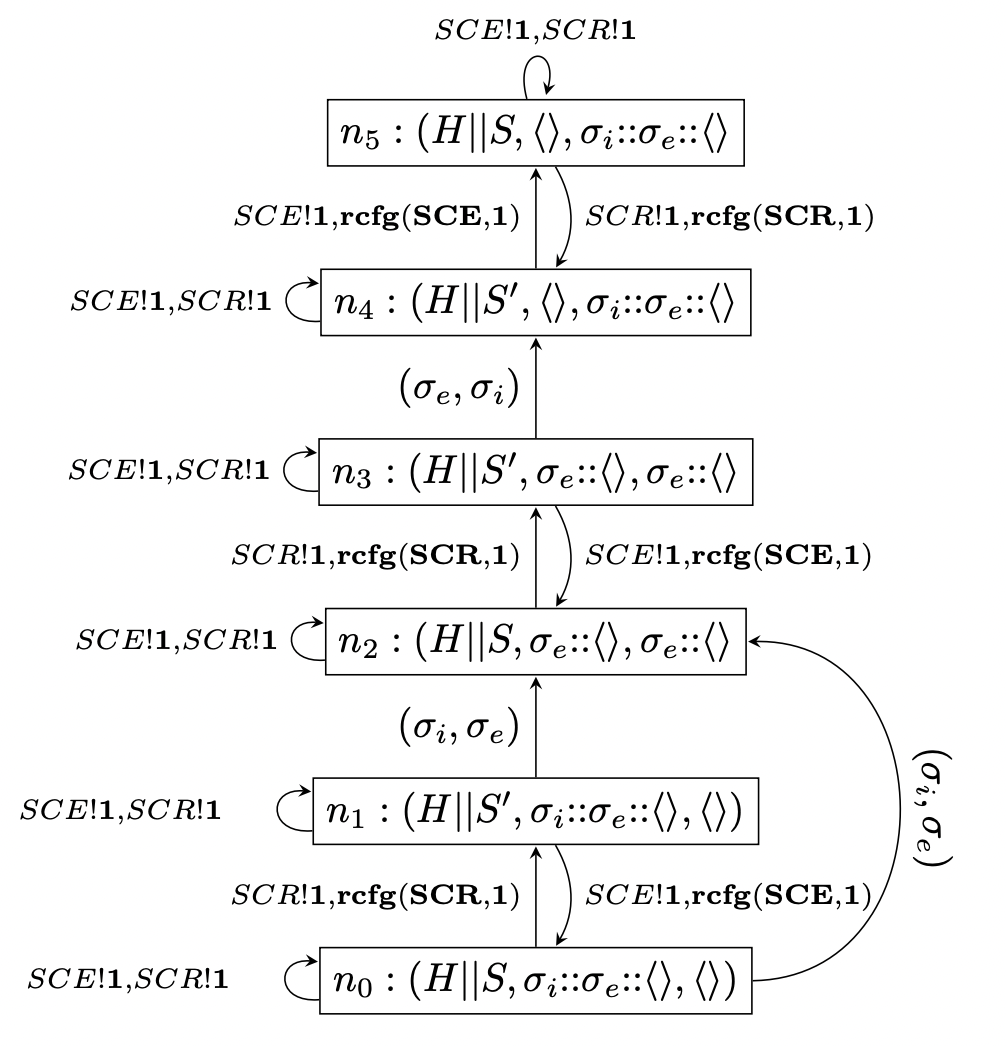
\includegraphics[width=0.8\textwidth]{firewall-lts.png}}
    \caption{سیستم انتقال برچسب‌دار برای شبکه‌ی دیوار آتش}
    \label{fig:dynetkat:lts}
\end{figure}
نمودار نمایش داده شده در شکل
\ref{fig:dynetkat:lts}
سیستم انتقال برچسب‌دار
\lf{Labeled Transition System}
این شبکه‌ را در حالتی که یک بسته روی پورت ورودی و یک بسته روی پورت خروجی شبکه وجود دارد نشان می‌دهد.
همانطور که در نمودار مشخص است، عملیات
$(\sigma_e,\sigma_i)$
که به معنای ارسال بسته از پورت ورودی به پورت خروجی است تنها در قسمتی از این سیستم انتقال قابل دسترسی است که پیش از آن یکی از عملیات‌های
$SCR?1$
یا
$rcfg(SCR,1)$
انجام شده باشند.
بنابراین در این حالت شبکه تنها در صورتی که بسته خارجی را به داخل ارسال می‌کند که پیش از آن پیام آغاز ارتباط امن دریافت کرده‌ باشد.


\section{ساختمان رویداد}
ساختمان رویداد%
\lf{Event Structure}
\cite{es}
یک مدل محاسباتی%
\lf{Computational Model}
غیر‌برگ‌برگ شده%
\lf{Non-Interleaving}
برای پردازه‌های هم‌روند%
\lf{Concurrent}
است.
در این مدل، برخلاف مدل‌های برگ‌برگ شده%
\lf{Interleaving}
مانند سیستم‌انتقال که هم‌روندی پردازه‌های موازی با انتخاب غیرقطعی مدل می‌شود، هم‌روندی پردازه‌ها به صورت صریح در مدل توصیف می‌شوند
\cite{sassone1996models}.
\begin{definition}{ساختمان رویداد}
    یک ساختمان رویداد یک سه‌تایی
    $(E,\#,\vdash)$
    است که در آن:
    \begin{enumerate}
        \item $E$
              یک مجموعه از رویداد‌ها است
        \item $\#$
              رابطه‌ی تعارض%
              \lf{Conflict}
              ، یک رابطه‌ی دودویی متقارن و غیربازتابی بر روی مجموعه‌ی
              $E$
              است
        \item $\vdash \subseteq Con \times E$
              رابطه‌ی فعال سازی%
              \lf{Enabling}
              است که شرط زیر را برقرار می‌کند:
              \begin{align*}
                  (X \vdash e) \wedge (X \subseteq Y \in Con)
                  \Rightarrow Y \vdash e
              \end{align*}
    \end{enumerate}
    در رابطه‌ی بالا
    $Con$
    (مخفف 
    Consistent
    )،
    زیرمجموعه‌ای از مجموعه‌ی توانی رویدادها است که اعضای آن فاقد تعارض باشند.
    به صورت دقیق‌تر داریم:
    \begin{align*}
        Con = \s{X \subseteq E ~|~ \forall e,e' \in X. \neg(e\#e')}
    \end{align*}
\end{definition}
\begin{definition}
    به ازای هر ساختمان رویداد، می‌توانیم رابطه‌ی فعال‌سازی مینیمال را به صورت زیر تعریف کنیم:
    \begin{align*}
        X \vdash_{min} e \iff X \vdash e \wedge
        ( \forall Y \subseteq X . Y \vdash e \Rightarrow Y = X )
    \end{align*}
    همچنین در هر ساختمان رویدادی شرط زیر برقرار است:
    \begin{align*}
        Y \vdash e \Rightarrow \exists X \subseteq Y . X \vdash_{min} e
    \end{align*}
\end{definition}

برای مشخص کردن وضعیت یک سیستم در هر لحظه از مفهومی به نام پیکر‌بندی%
\lf{Configuration}
استفاده می‌شود و
و یک مجموعه شامل رویدادهایی است که تا آن لحظه در سیستم رخ داده‌اند.
\begin{definition}
    \label{def:configuration}
    اگر
    $\mathrm{E} = (E,\#,\vdash)$
    یک ساختمان رویداد باشد، یک پیکربندی آن یک زیرمجموعه از رویداد‌ها
    $x \subseteq E$
    است که شرایط زیر را داشته باشد:
    \begin{enumerate}
        \item $x \in Con$
        \item $\forall e \in x. \exists e_0,...,e_n \in x. e_n = e \ \wedge
                  \forall i \leq n. \s{e_0,...,e_{i-1}} \vdash e_i$
    \end{enumerate}
\end{definition}
مجموعه‌ی همه‌ی پیکربندی‌های یک ساختمان رویداد مانند
$\mathrm{E}$
با
$\mathcal{F}(\mathrm{E})$
نمایش داده می‌شود.

شبکه‌ی موجود در شکل
\ref{fig:es:update}
را در نظر بگیرید.
در این شبکه دو میزبان ۱ و ۲ به صورت هم‌روند یک بسته را به سوییچ ارسال می‌کنند.
این بسته‌ها شامل اطلاعات برای به روزرسانی مسیر‌های دیگر در شبکه هستند، بنابراین سوییچ پس از دریافت هر دوی این بسته‌ها آن ها را پردازش کرده و مسیر‌های خود را به روزرسانی می‌کند.
فرض کنید رویدادهای 
$r_1$
و
$r_2$
به ترتیب مشخص کننده‌ دریافت یک بسته از میزبان ۱ و ۲ باشند و 
رویداد 
$u$
به‌روز رسانی سوییچ را مشخص کنند.
برای مدل کردن این شبکه می‌توانیم از یک ساختمان رویداد به صورت زیر استفاده کنیم:
\begin{align*}
    \mathrm{E} & = (
    \s{r_1,r_2,u},
    \e, \s{(\e,r_1),(\e,r_2),(\s{r_1,r_2},u)}
    )
\end{align*}
یکی از روش‌های رسم نمودار برای ساختمان رویداد، رسم نمودار هسه%
\lf{Hasse}
برای مجموعه‌ی پیکربندی‌های این ساختمان رویداد بر اساس رابطه‌ی زیرمجموعه است.
برای مثالی که بیان شد می‌توان نموداری مطابق شکل
\ref{fig:es:configs}
را رسم کرد.
\begin{figure}
    \centering
    \begin{tikzpicture}[scale=0.8]
        \crd{0}{0}{$\emptyset$}
        \crd[left]{-2}{1}{$\s{r_1}$}
        \crd[right]{2}{1}{$\s{r_2}$}
        \crd[right]{0}{2}{$\s{r_1,r_2}$}
        \crd[right]{0}{3}{$\s{r_1,r_2,u}$}
        \draw [ultra thick] (0,0) -- (2,1);
        \draw [ultra thick] (0,0) -- (-2,1);
        \draw [ultra thick] (-2,1) -- (0,2);
        \draw [ultra thick] (2,1) -- (0,2);
        \draw [ultra thick] (0,2) -- (0,3);
    \end{tikzpicture}
    \caption{}
    \label{fig:es:configs}
\end{figure}

\begin{figure}
    \centering
    \begin{tikzpicture}[node distance={15mm},minimum size=10mm,
            main/.style = {draw, circle}]
        \node[main] (S)  {$s$};
        \node[main] (H1) [above of=S,left of=S] {$h_1$};
        \node[main] (H2) [above of=S,right of=S] {$h_2$};
        \draw[->,thick] (H1) -- (S);
        \draw[<-,thick] (S) -- (H2);
    \end{tikzpicture}
    \caption{}
    \label{fig:es:update}
\end{figure}

\section{مدل علّی}
پیدا کردن تعریفی برای علت واقعی
\lf{Actual Cause}
مبحثی است که مورد مطالعه و تحقیق بسیاری قرار گرفته است.
این مساله به طور خاص در متون فلسفه مورد توجه قرار گرفته است.
یکی از تعاریف علت واقعی که مورد توجه بسیاری قراری گرفته است، تعریفی مبتنی بر وابستگی خلاف واقع
\lf{Counterfactual}
است.
مطابق این تعریف، رویداد الف علت رویداد ب است اگر در شرایطی که رویداد الف اتفاق نیافته باشد، رویداد ب هم اتفاق نیافتند.
در اینجا اتفاق نیفتادن رویداد الف خلاف واقع است، چون در سناریوی واقعی
(سناریو ای که واقعا اتفاق افتاده و مشاهده شده است)
رویداد الف اتفاق افتاده است و در نظر گرفتن شرایطی که در آن رویداد الف اتفاق نیفتاده باشد بر خلاف واقعیت موجود است.
اما این مدل به تنهایی امکان پیدا کردن علت مناسب را در همه‌ی موارد ندارد.
به عنوان مثال سناریوی زیر را در نظر بگیرید که در آن سارا و بهرام هر کدام یک سنگ را برداشته و به سمت یک بطری شیشه‌ای پرتاب می‌کنند.
در این سناریو، سنگ سارا زودتر از سنگ بهرام به بطری برخورد کرده و در نتیجه آن را می‌شکند.
در این سناریو واضح است که پرتاب سنگ توسط سارا علت شکسته شدن بطری است.
فرض کنید بخواهیم از علیت مبتنی بر خلاف واقع برای پیدا کردن این علت استفاده کنیم.
بنابراین باید شرایطی را در نظر بگیریم که سارا سنگ خود را پرتاب نکند.
اما مشکل اینجاست که در این شرایط همچنان بطری شکسته می‌شود، چون اگر سارا سنگ خود را پرتاب نکند، بهرام همچنان سنگ خود را پرتاب می‌کند و در نتیجه این بار سنگ بهرام به بطری برخورد کرده و آن را می‌شکند.
بنابراین در این سناریو امکان تعریف پرتاب سنگ توسط سارا به عنوان علت شکسته شدن بطری با استفاده از استدلال مبتنی بر خلاف واقع وجود ندارد.
هالپرن
\lf{Halpern}
و پرل
\lf{Pearl}
برای حل کردن مشکلاتی از این دست، تعریف جدیدی از علت واقعی
\cite{hp}
ارائه کردند.
مدل ارائه شده توسط آن‌ها به دلیل اینکه مبنای ریاضی دارد امکان استفاده از آن را در آنالیز و تحلیل سیستم‌های محاسباتی فراهم می‌کند.
به همین دلیل این تعریف در مقالات زیادی در حوزه‌ی دانش کامپیوتر مورد استفاده قرار گرفته است.
برای تعریف علت واقعی ابتدا برخی مفاهیم اولیه مورد استفاده در این تعریف توضیح داده می‌شوند.
به صورت کلی فرض می‌شود که دنیای مورد تحلیل توسط تعدادی متغیر تصادفی مدل شده است.
اگر
$X$
یک متغیر تصادفی باشد، یک رویداد به شکل
$X=x$
تعریف می‌شود.
برخی از این متغیر‌ها بر روی یکدیگر تاثیر گذارند.
این وابستگی‌ها در قالب مجموعه‌ای از معادلات ساختاری
\lf{Structural Equations}
مدل می‌شوند.
هر یک از این معادلات در واقع یک مکانیزم یا قانون مشخص در این دنیا را مدل می‌کنند.
متغیرها به دو دسته درونی
\lf{Endogenous}
و برونی
\lf{Exogenous}
تقسیم می‌شوند.
متغیر‌های برونی متغیر‌هایی در نظر گرفته می‌شوند که مقدار آن‌ها توسط عواملی که درون مدل نیستند تعیین می‌شوند.
بنابراین در یک مدل علی فرض می‌شود که مقدار این متغیر‌ها از قبل مشخص است.
اما متغیر‌های درونی متغیرهایی هستند که مقدار آن‌ها بر اساس معادلات ساختاری تعیین می‌شود.
به صورت دقیق‌تر، امضای
\lf{Signature}
یک مدل یک سه‌تایی
$\mc{S} = (\mc{U},\mc{V},\mc{R})$
است که در آن
$\mc{U}$
مجموعه‌ی متغیر‌های بیرونی
$\mc{V}$
مجموعه‌ی متغیر‌های درونی و
$\mc{R}$
دامنه‌ی مقادیر ممکن برای هر یک از متغیر‌ها را مشخص می‌کند.
در این مدل فرض می‌شود که مجموعه‌ی متغیر‌های درونی محدود است.
مدل علّی بر روی یک امضای
$\mc{S}$
یک دوتایی
$\mc{M} = (\mc{S},\mc{F})$
است که در آن
$\mc{F}$
به هر متغیر داخلی
$X \in \mc{V}$
یک تابع
$F_X: \times_{Z\in ((\mc{U}\cup \mc{V})\setminus \s{X})}R(Z)
\rightarrow \mathcal{R}(X)$
اختصاص می‌دهد.
نشانه‌گذاری
$\times_{Z\in ((\mc{U}\cup \mc{V})\setminus \s{X})}$
ضرب خارجی
\lf{Cross-Product}
مجموعه‌های
$\mc{R}(Z)$
را به ازای تمام متغیر‌هایی مانند 
$Z$
در 
$(\mc(U)\cup \mc{V}) \setminus \s{X}$
مشخص می کند.
بنابراین اگر فرض کنیم
$(\mc{U}\cup \mc{V})\setminus \s{X} = \s{Z_1,...,Z_k}$
، آنگاه 
$\times_{Z\in ((\mc{U}\cup \mc{V})\setminus \s{X})}\mc{R}(Z)$
متشکل از چندتایی‌هایی به شکل
$(z_1,...,z_k)$
است که به ازای 
$i = 1,...,k$
هر 
$z_i$
یک مقدار ممکن برای متغیر 
$Z_i$
است.
هر تابع، معادله‌ی یک متغیر را به ازای مقادیر تمام متغیر‌های دیگر مشخص می‌کند.
به عنوان مثال اگر فرض کنیم
$F_X(Y,Z,U) = Y + U$
اگر داشته باشیم
$Y=3, U=2$
آنگاه مقدار
$X$
برابر ۵ خواهد شد.
این معادلات امکان تفسیر آن‌ها بر اساس شرایط خلاف واقع را می‌دهند.
به عنوان مثال در همین مدل اگر فرض کنیم که
$U=u$
می‌توانیم نتیجه بگیریم که اگر مقدار متغیر
$Y$
برابر ۴ باشد آنگاه مستقل از اینکه مقدار بقیه‌ی متغیر‌ها در دنیای واقعی چه مقداری دارند، مقدار متغیر
$X$
برابر
$u+4$
خواهد بود که به صورت
$(M,u) \vDash [Y \la 4](X = u + 4)$
نوشته می‌شود.
توابع ذکر شده فقط برای متغیر‌های درونی تعریف می‌شوند و همانطور که پیش‌تر اشاره شد، برای متغیرهای بیرونی تابعی تعریف نمی‌شود و فرض می‌شود که مقدار آن‌ها از قبل مشخص شده است
\cite{Halpern_2016}.

\begin{example}
      \label{ex:hp:fire}
      یک جنگل را در نظر بگیرید که می‌تواند توسط رعد و برق یا یک کبریت رها شده دچار آتش سوزی شود.
      برای مدل کردن این سناریو از سه متغیر بولی
      \lf{Boolean}
      استفاده می‌کنیم:
      \begin{itemize}
            \item متغیر
                  $F$
                  که اگر جنگل دچار آتش سوزی شود مقدار آن درست است و در غیر این صورت مقدار آن غلط است
            \item متغیر
                  $L$
                  که اگر رعد و برق اتفاق افتاده باشد مقدار آن درست است و در غیر این صورت غلط است
            \item متغیر
                  $M$
                  که اگر یک کبریت در جنگل رها شده باشد مقدار آن درست است و در غیر این صورت غلط است
      \end{itemize}
\end{example}
در این مثال فرض می کنیم که مقادیر متغیر‌های برونی به گونه‌ای است که تمام شرایط لازم برای آتش سوزی جنگل در صورتی که رعد و برق اتفاق بیافتد یا کبریتی در جنگل رها شود را دارد
(به عنوان مثال درختان جنگل به اندازه‌ی کافی خشک هستند و اکسیژن کافی در هوا وجود دارد).
در این مدل تابع متغیر
$F$
را به گونه‌ای تعریف می‌کنیم که داشته باشیم:
$F_F(\vec u, L , M) = L \vee M$.
همانطور که پیش‌تر بیان شد، این مدل علّی امکان بررسی معادلات بر اساس شرایط خلاف واقع را می‌دهد.
به صورت دقیق‌تر اگر
$M = (\mc{S},\mc{F})$
یک مدل علی،
$\vec X$
یک بردار از متغیرهای درونی و
$\vec{x}, \vec{u}$
برداری از مقادیر متغیر‌های
$\vec{X},\mc{U}$
باشند
مدل
$M_{\vec{X}\la \vec{x}}$
را با امضای
$S_{\vec X}=(\mc{U},\mc{V}-\vec X,\mc{R}|_{\mc{V} \setminus \vec{X}})$
یک زیرمدل
\lf{Sub-Model}
از
$M$
تعریف می‌کنیم که در آن
$\mc{R}|_{\mc{V}\setminus \vec X}$
محدود کردن 
$\mc{R}$
به متغیر‌های داخل 
$\mc{V} \setminus \vec X$
است.
به صورت شهودی این مدل حاصل مداخله‌
\lf{Intervention}
ای در مدل
$M$
است که در آن مقادیر
$\vec{x}$
را به متغیر‌های
$\vec{X}$
اختصاص داده‌ایم.
به صورت دقیق‌تر تعریف می‌کنیم
$M_{\vec{X}\la\vec{x}} = (\mc{S}_{\vec{X}},\mc{F}^{\vec{X}\la\vec{x}})$
که
$F_Y^{\vec{X}\la\vec{x}}$
از تابع
$F_Y$
که در آن مقادیر
$\vec{x}$
را به متغیرهای
$\vec{X}$
اختصاص داده‌ایم به دست می‌آید.
به عنوان مثال اگر
$M$
مدل مثال
\ref{ex:hp:fire}
باشد آنگاه در مدل
$M_{L\la \F}$
معادله‌ی متغیر
$F$
به
$F = M$
تبدیل می‌شود.
این معادله دیگر به متغیر
$L$
وابسته نیست بلکه با توجه به مقدار آن که در اینجا غلط است معادله‌ی جدیدی دارد.
علاوه براین توجه کنید که در مدل
$M_{L\la \F}$
دیگر معادله‌ای برای متغیر
$L$
وجود ندارد.
توجه کنید که در حالت کلی ممکن است یک بردار یکتا از مقادیر متغیر‌ها برای یک مدل وجود نداشته باشد که همزمان تمامی معادلات را حل کند.
در مدل علّی یک بردار از مقادیر متغیر‌های برونی
$\vec u$
یک هم‌بافت
\lf{Context}
نامیده می‌شود.
در مدل‌های بازگشتی به ازای یک هم‌بافت مشخص همیشه یک راه‌حل یکتا برای تمامی معادلات مدل وجود دارد.
در ادامه فرض می‌شود که مدل‌ها بازگشتی هستند. تعمیم مدل‌ علّی برای مدل‌های غیربازگشتی در
\cite{hp}
توضیح داده است.
برای یک مدل می‌توان یک شبکه‌ی علّی ترسیم کرد.
این شبکه یک گراف جهت‌دار است که به ازای هر متغیر یک گره در آن وجود دارد و یک یال بین دو گره وجود دارد اگر تابع متغیر دوم به متغیر اول وابسته باشد.
به عنوان مثال شکل زیر شبکه‌ی علّی مثال
\ref{ex:hp:fire}
را نشان می‌دهد:
\begin{center}
      \begin{tikzpicture}[node distance={15mm}]
            \node (l) {L};
            \node (m) [below right of=l]  {M};
            \node (f) [above right of=m] {F};
            \node (u) [above right of=l] {U};
            \draw [->] (l) -- (m);
            \draw [->] (f) -- (m);
            \draw [->] (u) -- (l);
            \draw [->] (u) -- (f);
      \end{tikzpicture}
\end{center}
در ادامه برای سادگی رسم شبکه‌ی علی، متغیر‌های برونی را از آن‌ها حذف می‌کنیم.
\subsection{علت واقعی}
در ادامه‌ فرمول‌های لازم برای تعریف علت واقعی توصیف می‌شوند.
اگر
$\mc{S} = (\mc{U},\mc{V},\mc{R})$
یک امضا باشد فرمول
‍‍$X=x$
یک رویداد بدوی
\lf{Prime Event}
نامیده می‌شود که
‍$X \in \mc{V},x \in \mc{R}(X)$.
فرمول
$[Y_1 \la y_1,...,Y_k\la y_k]\varphi$
یک فرمول علّی پایه
\lf{Basic Causal Formula}
نامیده می‌شود که در آن:
\begin{itemize}
      \item $\varphi$
            یک ترکیب بولی از رویداد‌های بدوی است
      \item $Y_1,...,Y_k$
            متغیر‌های متمایز در
            $\mc{V}$
            هستند
      \item $y_i \in \mc{R}(Y_i)$
\end{itemize}
این فرمول به صورت خلاصه به شکل
$[\vec{Y}\la \vec{y}]\varphi$
نوشته می‌شود و اگر
$k=0$
باشد آنگاه به صورت
$\varphi$
نوشته می‌شود.
به صورت شهودی یک فرمول به شکل
$[\vec{Y}\la \vec{y}]\varphi$
بیان می‌کند که در شرایط خلاف واقع‌ ای که در آن مقادیر
$\vec{y}$
به متغیر‌های
$\vec{Y}$
اختصاص داده شده است فرمول
$\varphi$
برقرار است.
یک فرمول علّی به صورت یک ترکیب بولی از فرمول‌های علّی پایه تعریف می‌شود.
برقراری فرمول علی
$\psi$
در مدل
$M$
تحت هم‌بافت
$\vec u$
را به صورت
$(M,\vec u) \vDash \psi$
نشان می‌دهیم.
به عنوان مثال
$(M,\vec{u}) \vDash [\vec{Y}\la \vec{y}](X=x)$
برقرار است اگر مقدار متغیر
$X$
در راه حل معادلات مدل
$M_{\vec{Y}\la \vec{y}}$
تحت هم‌بافت
$\vec u$
برابر
$x$
باشد.

\begin{definition}
      \label{def:cause}
      فرمول
      $\vec X = \vec x$
      علت واقعی
      $\varphi$
      (
      که تاثیر
      \lf{Effect}
      نامیده می‌شود)
      در
      $(M,\vec{u})$
      است
      اگر شرایط زیر برای آن برقرار باشد:
      \begin{enumerate}
            \item $(M,\vec{u}) \vDash (\vec{X} = \vec{x}) \wedge \varphi$
            \item یک افراز مانند
                  $(\vec{Z},\vec{W})$
                  از مجموعه‌ی متغیر‌های
                  $\mc{V}$
                  با شرط
                  $\vec{X} \subseteq \vec{Z}$
                  و مقادیر
                  $(\vec{x},\vec{w}')$
                  برای متغیر‌های
                  $(\vec{X},\vec{W})$
                  وجود داشته باشد که داشته باشیم
                  $(M,\vec{u})\vDash \vec{Z} = \vec{z}^*$
                  و شرایط زیر را برآورده کند:
                  \begin{enumerate}
                        \item $(M,\vec u)\vDash[\vec{X}\la\vec{x}',\vec{W}\la\vec{w}']
                                    \neg \varphi$
                        \item $\forall \vec{W'} \subseteq \vec{W},\vec{Z'}\in \vec{Z}.
                                    (M,\vec{u})\vDash [\vec X\la\vec x,\vec{W}'\la \vec{w}',\vec{Z}'\la \vec{z}^*]\varphi$
                  \end{enumerate}
            \item $\vec X$
                  مینیمال باشد.
      \end{enumerate}
\end{definition}
در این تعریف شرط اول بیان می‌کند که علت و تاثیر هر دو در شرایط واقعی برقرار هستند.
شرط دوم به دنبال پیدا کردن شرایطی است که تحت آن تاثیر به صورت غیر واقع به علت وابسته باشد.
این شرایط متغیرهای
$\vec W$
و مقادیری مانند
$\vec{w}'$
برای آن‌ها هستند.
شرط ۲.آ بررسی می‌کند که تحت شرایطی که توسط
$\vec W \la \vec{w}'$
به وجود می‌آید اگر علت مقداری متفاوت از مقدار خود در هم‌بافت واقعی داشته باشد اثر در مدل دیده نمی‌شود.
شرط ۲.ب بررسی می‌کند که شرایط
استفاده شده در ۲.آ عامل
از بین رفتن اثر در ۲.آ نباشند.
برای این منظور در شرایطی که علت مقدار واقعی خود را دارد در تمامی حالت‌هایی که متغیر‌های شرایط می‌توانند داشته باشند بررسی می‌شود که اثر همچنان برقرار باشد.
شرط سوم در واقع بیان می‌کند که زیرمجموعه‌ای از علت وجود نداشته باشد که همزمان شرایط ۱ و ۲ را برقرار کند.
در تعریف بالا
$(\vec W, \vec w',\vec x')$
یک شاهد
\lf{Witness}
بر اینکه
$\vec X = \vec x$
علت
$\varphi$
است تعریف می‌شود.

\subsection{پیدا کردن علت واقعی در مسائل}

در ادامه مثال سارا و بهرام که در ابتدای این بخش ذکر شده بود را بررسی می‌کنیم.

برای مدل کردن این مساله متغیر‌های زیر را در نظر می‌گیریم:
\begin{itemize}
      \item $BT$:
            پرتاب سنگ توسط بهرام
      \item $BH$
            برخورد سنگ بهرام به بطری
      \item $ST$:
            پرتاب سنگ توسط سارا
      \item $SH$:
            برخورد سنگ سارا به بطری
      \item $BS$:
            شکسته شدن بطری
\end{itemize}

\begin{figure}
      \centering
      \begin{tikzpicture}[node distance={15mm}]
            \node (bs)  {$BS$};
            \node (sh) [above left of=bs] {$SH$};
            \node (bh) [below left of=bs] {$BH$};
            \node (st) [left of=sh]{$ST$};
            \node (bt) [left of=bh] {$BT$};
            \draw [->] (st) -- (sh);
            \draw [->] (sh) -- (bh);
            \draw [->] (bt) -- (bh);
            \draw [->] (sh) -- (bs);
            \draw [->] (bh) -- (bs);
      \end{tikzpicture}
      \caption{}
      \label{fig:hp:sb}
\end{figure}
ابتدا فرض می‌کنیم که متغیر‌های
$BT,ST$
تنها به متغیر‌های برونی وابسته‌اند.
بطری در صورتی شکسته می‌شود که هر یک از سنگ‌های سارا یا بهرام با آن برخورد کنند.
بنابراین برای شکسته شدن بطری معادله‌ی
$BS = BH \vee SH$
را در نظر می‌گیریم.
نکته‌ی اصلی در این مساله این است که سنگ سارا زودتر از سنگ بهرام به شیشه برخورد می‌کند، به همین دلیل لازم است تا این موضوع در مدل لحاظ شود.
یک راه برای مدل کردن این مساله این است که معادله‌ی برخورد سنگ بهرام به شیشه را به گونه‌ای تعریف کنیم که تنها در صورتی که سنگ سارا به بطری برخورد نکرده باشد آنگاه سنگ بهرام به بطری برخورد کند.
بنابراین می‌توانیم معادله‌ی
$BH = BT \wedge \neg SH$
را تعریف کنیم.
علاوه بر این معادله‌ی برخورد سنگ سارا را بدون وابستگی به برخورد سنگ بهرام تعریف می‌کنیم:
$SH = ST$.
با توجه به این تعاریف برای معادلات می‌توانیم گراف علّی شکل
\ref{fig:hp:sb}
را برای این مدل رسم کنیم
در این مدل می‌توانیم
$ST = \T$
را به عنوان علت
$BS = \T$
تعریف کنیم.
برای برقراری شرط ۲ در تعریف علت واقعی شرایط
$\vec W = \s{BT}$
و
$w' = \F$
را در نظر می‌گیریم.
در این شرایط چون مقدار
$BH$
برابر
$\F$
می‌شود، مقدار
$BS$
تنها وابسته به مقدار
$SH$
و در نتیجه
$ST$
می‌شود.
همچنین در این مدل
$BT = \T$
علت شکسته شدن شیشه نیست.
مثلا فرض کنید که شرایط
$\vec W = \s{ST},w' = \F$
را در نظر بگیریم.
در این شرایط اگر مقدار
$BT$
را به
$\F$
تغیر دهیم مقدار
$BS$
هم غلط می‌شود.
بنابراین شرط ۲.آ برقرار است.
اما به ازای
$\vec Z' = \s{BH}$
شرط ۲.ب برقرار نمی‌شود.
در این حالت داریم:
$(M,\vec{u})\vDash[BT \la \T,ST \la \F,BH \la F]BS = \F$
توجه کنید با وجود اینکه مقدار درست به
$BT$
اختصاص یافته اما چون مقدار
$BH$
به مقدار آن در هم‌بافت واقعی برگردانده می‌شود در نتیجه مقدار
$BS$
همچنان غلط می‌ماند.

مثال بالا نشان می‌دهد که این تعریف از علت واقعی برخی از مشکلات موجود در تعاریف ساده مبتنی بر خلاف واقع را برطرف می‌کند و می‌تواند توضیح مناسبی در برخی از این مثال‌ها پیدا کند.
نکته‌ای که باید به آن توجه شود این است که هنوز روش یا معیاری برای این که چه تعریفی از علت واقعی تعریف مناسب است وجود ندارد.
تنها روش ممکن مقایسه تعاریف مختلف استفاده از آن‌ها در مساله‌ها و سناریوهای مختلف و بررسی تطابق علت به دست آمده با استفاده از این تعریف‌ها با شهود موجود از مساله است.

\subsection{مدل تعمیم‌یافته}
مدل علّی تعمیم یافته
\lf{Extended Causal Model}
یک سه‌تایی
$(\mc{S},\mc{F},\mc{E})$
است که
$(\mc{S},\mc{F})$
یک مدل علّی است و
$\mc{E}$
یک مجموعه از مقداردهی‌های مجاز
\lf{Allowable Settings}
برای متغیر‌های درونی است.
به صورت دقیق‌تر اگر متغیر‌های درونی
$X_1,...,X_n$
باشند آن‌گاه
$(x_1,...,x_n) \in \mc{E}$
اگر
$X_1=x_1,...,X_n=x_n$
یک مقداردهی مجاز است.
یک مقداردهی دلخواه به یک زیرمجموعه از متغیر‌های درونی مجاز است اگر امکان تعمیم به یک مقداردهی مجاز در
$\mc{E}$
را داشته باشد.
هدف از این تعریف جلوگیری از در نظر گرفتن علت‌هایی است که شرایط رخ دادن آن‌ها غیر محتمل است.
با توجه به تعریف مقداردهی مجاز، علت واقعی در یک مدل تعمیم یافته به گونه‌ای تعریف می‌شود که در شرط ۲ فقط امکان مقداردهی‌های مجاز وجود داشته باشد.
در
\cite{hp}
تعریف دقیق علت واقعی در مدل تعمیم یافته بیان نشده است.
در بخش بعدی تعریفی از علت واقعی در مدل تعمیم یافته ارائه می‌شود.

\subsection{علت واقعی بدون شرط}
فرض کنید که
$\vec X = \vec x$
یک علت واقعی برای
$\varphi$
در
$(M,\vec u)$
با استفاده از شاهد
$(\e,\e,\vec x')$
باشد.
با توجه به اینکه در اینجا
$\vec W$
یک بردار خالی است پس عملا شرط ۲.ب به بررسی شرط زیر تبدیل می‌شود:
\begin{align*}
      \forall \vec{Z'}\in \vec{Z}.
      (M,\vec{u})\vDash [\vec X\la\vec x,\vec{Z}'\la \vec{z}^*]\varphi
\end{align*}
با دقت در شرط بالا می‌توان دریافت که مقدار متغیر‌ها در فرمول‌های
$[\vec X\la\vec x,\vec{Z}'\la \vec{z}^*]\varphi $
با مقدار متغیر‌ها در هم‌بافت اولیه تفاوتی ندارد زیرا مقدار آن‌ها به مقداری که در هم‌بافت اولیه داشته‌اند برگردانده می‌شود.
بنابراین در شرط بالا می‌توان نتیجه گرفت:
\begin{align*}
      (M,\vec{u})\vDash [\vec X\la\vec x,\vec{Z}'\la \vec{z}^*]\varphi 
      \iff (M,\vec{u}) \vDash \varphi
\end{align*}
بنابراین شرط ۲.ب معادل با شرط ۱ می‌شود.
با توجه به این موضوع می‌توان قضیه زیر را نتیجه گرفت:
\begin{proposition}
      \label{prop:but-for}
     اگر 
     $\vec X = \vec x$
     در 
     $(M,\vec u)$
     با شاهدی به شکل
     $(\e,\e,\vec x')$
     شرط‌های ۱، ۲.آ و ۳ در تعریف 
     \ref{def:cause}
     را برای 
     $\varphi$
     برآورده کند آنگاه 
     $\vec X = \vec x$
     یک علت واقعی برای 
     $\varphi$
     در 
     $(M,\vec u)$
     است.
\end{proposition}


% !TeX root=../../../main.tex
\chapter{مروری بر کار‌های پیشین}
%\thispagestyle{empty} 
توضیح خطا
\lf{Fault Explanation}
و
متمرکز کردن خطا
\lf{Fault Localization}
روش‌هایی هستند
که فرآیند رفع‌ایراد نرم‌افزار را تسهیل می‌کنند.
توضیح‌خطا روش‌هایی را شامل می‌شود که به کاربر کمک می‌کند که با استفاده از یک مثال‌نقض یا یک دنباله از اجرای سیستم به ماهیت خطا و در نتیجه روش اصلاح خطا پی ببرد.
در روش‌های متمرکز کردن خطا هدف مشخص کردن بخشی از سیستم است که عامل خطا بوده و امکان اندازه‌گیری کمی و مقایسه آن با دیگر بخش‌ها وجود دارد
\cite{groce2006error}.
یکی از روش‌های توضیح خطا پیدا کردن علت خطا بر اساس استدلال مبتنی بر خلاف واقع که توسط لوئیس در
\cite{lewis1973counterfactuals}
ارائه شده می‌باشد که در پژوهش‌هایی مانند
\cite{zeller2009programs,groce2006error,groce2003went}
استفاده شده است.
هالپرن و پرل در
\cite{hp}
تعریفی مبتنی بر استدلال خلاف واقع لوئیس ارائه کردند که توانسته است برخی از مشکلات تعریف لوئیس در پیدا کردن علت در سناریو‌های پیچیده را بر طرف کند.
در ادامه برخی از پژوهش‌هایی که از تعریف هالپرن و پرل برای توضیح خطا استفاده کرده‌اند را مورد بررسی قرار می‌دهیم.

\section{تخمین پوشش}
در
\cite{Chockler_Halpern_Kupferman_2008}
نویسندگان از مدل
HP
برای تخمین میزان پوشش
\lf{Covering}
سیستم توسط یک توصیف در فرآیند وارسی مدل استفاده کرده‌اند.
معیارهای پوشش معمولا در فرآیند تست سیستم استفاده می‌شوند و مشخص کننده‌ درصدی از اجزا یا حالت‌های سیستم هستند که توسط مجموعه‌ی تست‌ها مورد استفاده یا بازدید قرار می‌گیرند.
در فرآیند وارسی مدل همه‌ی حالت‌های سیستم بررسی می‌شوند به همین دلیل در این شرایط اگر تغییر یک حالت منجر به نقض ویژگی توصیف شده شود این حالت پوشش داده شده توسط ویژگی تعریف می‌شود.
با استفاده از مفهوم مسئولیت
\lf{Responsiblity}
که در
\cite{hp2}
تعریف شده است، نویسندگان این پژوهش به جای در نظر گرفتن مقدار ۰ و ۱ برای پوشیده شدن یا نشدن از درجه‌ی مسئولیت استفاده می‌کنند.
همانطور که مشخص است این پژوهش به اصلاح و بهبود توصیف ویژگی کمک می‌کند و نه پیدا کردن علت خطا.
در این پژوهش همانند پژوهش جاری به شکل مستقیم از تعریف 
HP
استفاده شده است.

\section{علت خطا در مثال نقض}
در
\cite{chockler}
نویسندگان سیستم را به صورت یک سیستم انتقال
\lf{Transition System}
در نظر می‌گیرند که در آن هر حالت یک نگاشت از یک مجموعه‌ی متغیر‌های بولی به مقادیر درست و غلط است.
در این پژوهش با استفاده از تعریف علت واقعی در یک مثال نقض یک ویژگی توصیف شده در
LTL
\lf{Linear Temporal Logic}
یک دوتایی‌ متغیر و حالت به عنوان علت واقعی در نظر گرفته می‌شود.
در همین پژوهش یک الگوریتم تقریبی برای پیدا کردن همه‌ی علت‌ها در یک مثال نقض داده شده ارائه شده است و ابزاری برای نمایش این علت‌ها به صورت گرافیکی به کاربر توسعه داده شده و در ابزار درستی‌سنجی
RuleBase PE
متعلق به
IBM
گنجانده شده است.
\begin{figure}
    \centering
    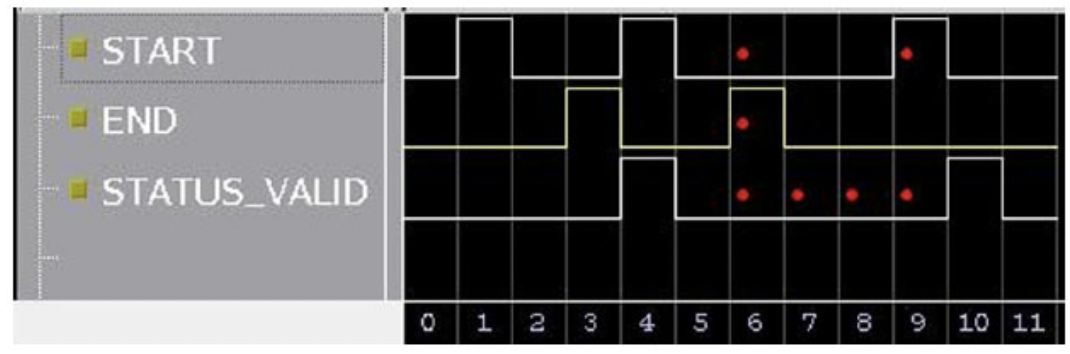
\includegraphics[width=15cm]{chockler.png}
    \caption{رابط کاربری ابزار
        RuleBase PE
    }
    \label{fig:rulebase}
\end{figure}
تصویر
\ref{fig:rulebase}
رابط کاربری ابزار 
RuleBase PE
را پس از پیدا کردن یک مثال نقض برای ویژگی زیر نشان می‌دهد:
\begin{align*}
    \boldsymbol{\mr{G}}((\neg \texttt{START} \wedge \neg \texttt{STATUS\_VALID} \wedge \texttt{END}) 
    \ra [\neg \texttt{START}\ \boldsymbol{\mr{U}}\ \texttt{STATUS\_VALID}])
\end{align*}
در این تصویر نقاط قرمز علت‌های واقعی هستند که با الگوریتم تقریبی پیاده‌سازی شده پیدا شده‌اند.
 این پژوهش یکی از کاربردی‌ترین استفاده‌ها از توضیح خطا و پیدا کردن علت خطا را نشان می‌دهد. 
در این پژوهش سعی شده است تا علت خطا در یک مثال نقض پیدا شود و به همین دلیل مقدار متغیر‌ها در حالت‌ها به عنوان علت پیدا می‌شوند در حالی که در پژوهش جاری هدف پیدا کردن علت خطا در کل سیستم است و در واقع ساختار‌های سیستم، مثلا وجود یا عدم وجود روابط تعارض یا فعال‌سازی به عنوان علت خطا پیدا می‌شوند.
اما همانند پژوهش جاری در این پژوهش هم به شکل مستقیم و بدون تغییر از تعریف 
HP
استفاده شده است.

\section{چک کردن علیت}
در پژوهش 
\cite{causality-checking}
نویسندگان تعریفی از علت‌ واقعی که الهام گرفته از تعریف 
HP
است ارائه می‌کنند و الگوریتم آن‌ها بر اساس این تعریف در حین اجرای فرآیند وارسی مدل
\lf{Model Checking}
علت‌ها را پیدا کرده و در نتیجه در انتهای وارسی مدل اگر سیستم ویژگی مورد نظر را نقض کرد به جای برگرداندن یک مثال نقض، رویداد‌هایی که علت رخداد خطا بوده‌اند را بر می‌گرداند.
در این پژوهش یک منطق برای توصیف یک دنباله از رویداد عملیات‌های سیستم ارائه شده است و فرمول‌های این منطق به عنوان علت خطا در نظر گرفته می‌شوند. 
این پژوهش هم همانند
\cite{chockler}
سعی بر پیدا کردن همه‌ی علت‌های بروز خطا دارد و علت‌ها عملا دنباله‌هایی از اجرای سیستم هستند. 
تفاوت اصلی این کار با پژوهش جاری در این است که در این پژوهش علت خطا در رفتارهای سیستم جستجو می‌شود در حالی که در پژوهش جاری علت خطا در میان عناصر ساختاری سیستم جستجو می‌شود.
این روش تنها برای ویژگی‌های دسترس‌پذیری ارائه شده است.
در
\cite{Caltais-LTL}
نویسندگان این روش‌ را برای ویژگی‌های دلخواه توصیف شده توسط
LTL
تعمیم دادند.

\section{علت واقعی در خودکاره‌های زمان‌دار}
در
\cite{kolbl2020dynamic}
نویسندگان از تعریف 
HP
برای پیدا کردن علت خطا در خودکاره‌های زمان‌دار
\lf{Timed Automata}
استفاده کرده‌اند.
در درستی‌سنجی خودکاره‌های زمان‌دار یک ابزار وارسی مدل بلا درنگ نقض ویژگی‌ را در قالب یک رد تشخیصی زمان‌دار 
\lf{Timed Diagnostic Trace}
که در واقع یک مثال‌نقض است بر می‌گرداند.
یک 
TDT
در واقع یک دنباله متناوب از انتقال تاخیر
\lf{Transition Delay}
و
انتقال عملیات
\lf{Delay Transition}
ها است که در آن مقدار تاخیر‌ها به صورت سمبلیک مشخص شده‌اند.
هدف این پژوهش پیدا کردن مقادیری یا دامنه‌ای از مقادیر برای این تاخیر‌های سمبلیک است که بروز خطا را اجتناب ناپذیر می‌کنند یا به عبارت دیگر علت واقعی هستند.
در این پژوهش اما به صورت مستقیم از تعریف 
HP
استفاده نشده است و بر اساس آن تعریفی برای علت واقعی نقض ویژگی در یک 
TDT
بیان شده است.

\section{چارچوب علیت بر اساس رد سیستم}
در 
\cite{gossler2013general}
نویسندگان این مساله را مطرح می‌کنند که تعریف ارائه شده توسط هالپرن و پرل ذاتا یک مدل بر اساس منطق گزاره‌ای
\lf{Propositional Logic}
است و به همین دلیل برای درستی‌سنجی پردازه‌ها ایده‌آل نیست.
در این پژوهش یک فرمالیسم و تعریف جدید برای علیت بر اساس تعریف 
HP
ارائه می‌شود که در آن از رد‌
\lf{Trace}
های سیستم به جای متغیر‌ها در مدل 
HP
استفاده می‌شود و امکان ترکیب
\lf{Composition}
چند مدل با یکدیگر را فراهم می‌کند.


\section{استدلال مبتنی بر علیت در 
HML
}
در
\cite{decomposing}
نویسندگان از مفهوم استدلال مبتنی در سیستم‌انتقال برچسب‌دار
\lf{Labeled Transition System}
و 
HML
\lf{Hennesy Milner Loigc} \cite{hml}
استفاده کرده‌اند.
در این پژوهش سیستم با استفاده از یک سیستم انتقال برچسب‌دار مدل می‌شود و رفتار ناامن توسط یک فرمول در قالب
HML
توصیف می‌شود.
سپس یک تعریف جدید که برگرفته شده از تعریف
HP
است با استفاده از این مدل‌ها برای علت واقعی بیان می‌شود.
در این تعریف از مفهومی به نام عدم‌وقوع
\lf{Non-Occurrence}
رویدادها که پیش‌تر در 
\cite{causality-checking}
مطرح شده بود استفاده می‌شود.
شهود کلی مفهوم عدم‌وقوع در علیت این است که در کنار اینکه رخ‌دادن برخی از رویداد‌ها منجر به خطا می‌شود، رخ ندادن رویداد‌ها هم می‌تواند به عنوان علت در نظر گرفته شود.
در تعریف ارائه شده در این پژوهش مجموعه‌ای از محاسبه‌
\lf{Computation}
های سیستم به عنوان علت برقراری یک فرمول 
HML
در سیستم که رفتار نا امن
\lf{Unsafe Behavior}
را توصیف می‌کند تعریف می‌شود.
هر محاسبه شامل یک دنباله از عملیات‌های سیستم در کنار تعدادی عملیات دیگر، که عدم وقوع آن‌ها هم جزئی از علت است، در نظر گرفته می‌شود.
به عبارت دیگر یک محاسبه را می‌توان شامل دو جز در نظر گرفت.
جز اول یک اجرای سیستم است که منجر به خطا می‌شود.
جز دوم مجموعه‌ای از اجراهای سیستم‌ است که منجر به خطا نمی‌شوند و حاصل برگ‌برگ‌ شدن
\lf{Interleaving}
برخی از عملیات‌ها در جز اول این محاسبه هستند.
عملیات‌های برگ‌برگ شده عملیات‌هایی هستند که عدم وقوع آن‌ها به عنوان علت بروز 
خطا در نظر گرفته می‌شود.
در این تعریف علت‌ واقعی به گونه‌ای تعریف شده است که محاسباتی‌ که منجر به فعال شدن فرمول 
HML
در سیستم می‌شوند به عنوان علت در نظر گرفته می‌شوند.
در این تعریف شروطی مشابه با شروط موجود در تعریف 
HP
در نظر گرفته شده است.
در 
\cite{causal-hml}
نویسندگان تعریف خود را بهبود دادند تا تطابق بیشتری با تعریف 
HP
داشته باشد.
علاوه بر این در این پژوهش ثابت شده است که این تعریف از علت در سیستم‌هایی که ارتباط همگام
\lf{Synchronized}
شده دارند قابل ترکیب نیست ولی در حالتی که سیستم‌ها ارتباط همگام نداشته باشند امکان ترکیب یا شکستن آن وجود دارد.
نتایج حاصل از این پژوهش یکی از انگیزه‌های اصلی پژوهش جاری بود برای اینکه با انتخاب یک مدل معنایی یا تعریف علیت متفاوت امکان ترکیب آن برای سیستم‌های همگام شده بررسی شود.
در ادامه به بررسی شباهت‌ها و تفاوت‌های این پژوهش و پژوهش جاری می‌پردازیم
اولا در این پژوهش تعریف جدیدی از علت واقعی ارائه شده است در حالی که در پژوهش جاری مستقیما از تعریف ارائه شده در
\cite{hp}
استفاده شده است.
در پژوهش جاری تمرکز بر پیدا کردن یک علت برای بروز خطا در سیستم است در حالی که در این پژوهش همه‌ی علل خطا مورد بررسی قرار می‌گیرند.
پژوهش جاری علل خطا را در ساختار‌های سیستم جستجو می‌کند در حالی که این پژوهش در میان رفتار‌های سیستم به دنبال علل خطا می گردد.

\section{جمع‌بندی}
همان طور که بررسی شد پژوهش‌های متعددی در زمینه‌ی توضیح خطا ارائه شده است که نشان از اهمیت این مساله در فرآیند درستی‌سنجی و اشکال‌زدایی دارد.
همچنین تعریف 
HP
هم مورد توجه زیادی برای پیدا کردن علت خطا قرار گرفته است.
یکی از مهم‌ترین تمایز‌های پژوهش جاری با پژوهش‌های پیشین در المان‌هایی است که در آن علت خطا پیدا می‌شود. 
همانطور که بررسی شد در تمامی پژوهش‌های پیشین در این زمینه علت خطا در میان رفتارهای سیستم جستجو می‌شود. 
اما در پژوهش جاری رویکردی متفاوت استفاده شده است و علت خطا در میان ساختار‌های سیستم، مثلا هم‌روند بودن یا نبودن پردازه، انجام می‌شود.
مساله‌ی دیگری که باید به آن اشاره شود این است که در پژوهش جاری همانند
\cite{chockler,Chockler_Halpern_Kupferman_2008}
به شکل مستقیم و بدون تغییر از تعریف 
HP
استفاده می‌شود.
% !TeX root=../main.tex
\chapter{روش و راه‌حل پیشنهادی}
%\thispagestyle{empty} 
\section{مقدمه}
در این فصل روش پیدا کردن علت خطا در شبکه‌های نرم‌افزاری توضیح داده می‌شود.
در بخش اول معنای عبارات نت‌کت پویا با استفاده از ساختمان رویداد تعریف می‌شود.
در بخش دوم یک مدل علّی برای توصیف ساختمان رویداد مطرح می‌شود.
در نهایت بخش سوم شامل استفاده از این روش‌ها برای توضیح خطا در شبکه‌های نرم‌افزاری با استفاده از چند مثال بیان می‌شود.


\section{مدل معنایی عبارات نت‌کت پویا در قالب ساختمان رویداد}
در این بخش ابتدا انواع ترکیب و محدود‌سازی ساختمان‌‌های رویداد تعریف می‌شود.
سپس با استفاده از این تعاریف  یک مدل معنایی برای عبارات نت‌کت پویا ارائه می‌شود.

\begin{definition}
    فرض کنید
    $\mr{E} = (E,\#,\vdash)$
    یک ساختمان رویداد باشد.
    به ازای یک مجموعه‌ی
    $A \subseteq E$
    ،
    محدودیت
    \lf{Restriction}
    $\mr{E}$
    به
    $A$
    یک ساختمان رویداد به شکل زیر است:
    \begin{align*}
        \mr{E} \lceil A = (A,\#_A,\vdash_A)
    \end{align*}
    که اگر 
    $Con_A$
    مجموعه‌ی تمامی زیرمجموعه‌های بدون تعارض 
    $A$ 
    در 
    $\mr{E}\lceil A$
    باشد آنگاه داشته باشیم:
    \begin{align*}
        X \subseteq Con_A & \iff X \subseteq A \wedge X \in Con                 \\
        X \vdash_A e      & \iff X \subseteq A \wedge e \in A \wedge X \vdash e
    \end{align*}
\end{definition}

\begin{definition}
    فرض کنید
    $\mr{E} = (E,\#,\vdash)$
    یک ساختمان رویداد و
    $a$
    یک رویداد باشد.
    ساختمان رویداد
    $a\mr{E} = (E',\#',\vdash')$
    که به معنای افزودن رویداد 
    $a$
    به عنوان پیشوند
    به 
    $\mr{E}$
    است
    به گونه‌ای تعریف می‌شود که داشته باشیم:
    \begin{align*}
         & E' = \s{(0,a)} \cup \s{(1,e)|e \in E},                                                                               \\
         & e_0' \#' e_1'  \iff \exists e_0,e_1.e_0' = (1,e_0)
        \ \wedge \ e_1' = (1,e_1) \ \wedge \ e_0 \# e_1                                                                         \\
         & X \vdash' e' \iff e' = (0,a) \text{ or } [e' = (1,e_1) \ \wedge \ (0,a)\in X \ \wedge \ \s{e|(1,e)\in X} \vdash e_1]
    \end{align*}
\end{definition}

\begin{definition}
    یک ساختمان رویداد برچسب‌دار
    \lf{Labeled Event Structure}
    یک پنج‌تایی به شکل
    $(E,\#,\vdash,L,l)$
    است که در آن
    $(E,\#,\vdash)$
    یک ساختمان رویداد،
    $L$
    یک مجموعه از برچسب‌ها
    (فاقد عنصر *
    \footnote{
        در ادامه از * برای مشخص کردن رویداد‌های ناهمگام استفاده می‌کنیم. به همین دلیل این عنصر را به عنوان یک برچسب خاص از مجموعه‌ی برچسب‌های ممکن کنار می‌گذاریم.
    }
    )
    و
    $l$
    یک تابع به فرم
    $l: E \ra L$
    است که به هر رویداد یک برچسب اختصاص می‌دهد.
    یک ساختمان رویداد برچسب‌دار را به اختصار به صورت
    $(\mr{E},L,l)$
    نشان می‌دهیم.
\end{definition}

\begin{definition}
    در یک ساختمان رویداد رابطه‌ی
    $\doublevee$
    را به صورت زیر تعریف می‌کنیم:
    \begin{align*}
        e \doublevee e' \iff e \# e' \vee e = e'
    \end{align*}
\end{definition}

\begin{definition}
    فرض کنید
    $(\mr{E},L,l)$
    یک ساختمان رویداد برچسب‌دار و
    $\alpha$
    یک برچسب باشد.
    $\alpha(\mr{E},L,l)$
    را به صورت یک ساختمان رویداد برچسب‌دار به شکل
    $(\alpha \mr{E},L',l)$
    تعریف می‌کنیم که در آن
    $L' = \s{\alpha}\cup L$
    و به ازای هر
    $e' \in E'$
    داشته باشیم:
    $$
        l'(e') = \begin{cases}
            \alpha & \text{ if } e = (0,\alpha) \\
            l(e)   & \text{ if } e = (1,e)
        \end{cases}
    $$
\end{definition}

\begin{definition}
    فرض کنید
    $\mr{E}_0 = (E_0,\#_0,\vdash_0,L_0,l_0)$
    و
    $\mr{E}_1 = (E_1,\#_1,\vdash_1,L_1,l_1)$
    دو ساختمان رویداد برچسب‌دار باشند.
    مجموع این دو ساختمان رویداد
    $\mr{E}_0 + \mr{E}_1$
    را به صورت یک ساختمان رویداد برچسب‌دار
    $(E,\#,\vdash,L,l)$
    تعریف می‌کنیم که در آن داشته باشیم:
    \begin{align*}
        E = \s{(0,e)|e \in E_0} \cup \s{(1,e)|e \in E_1}
    \end{align*}
    با استفاده از این مجموعه از رویداد‌ها توابع
    $\iota_k: E_k \ra E$
    را به ازای
    $k=0,1$
    به شکل زیر تعریف می‌کنیم:
    \begin{align*}
        \iota_k(e) = (k,e)
    \end{align*}
    رابطه‌ی تعارض را به گونه‌ای تعریف می‌کنیم که داشته باشیم:
    \begin{align*}
        e \# e' \iff & \exists e_0,e_0'. e = \iota_0(e_0)
        \wedge e' = \iota_0(e_0') \wedge e_0 \#_0e_0'             \\
                     & \bigvee \exists e_1,e_1'. e = \iota_1(e_1)
        \wedge e' = \iota_1(e_1') \wedge e_1 \#_1 e_1'            \\
                     & \bigvee \exists e_0,e_1.(e=\iota_1(e_0)
        \wedge e' =\iota_1(e_1)) \vee
        (e'=\iota_1(e_0) \wedge e =\iota_1(e_1))
    \end{align*}
    رابطه‌ی فعال‌سازی را به گونه‌ای تعریف می‌کنیم که داشته باشیم:
    \begin{align*}
        X \vdash e \iff & X \in Con \wedge e \in E \wedge                   & \\
                        & (\exists X_0 \in Con_0,e_0 \in E_0.X = \iota_0X_0
        \wedge e = \iota_0(e_0) \wedge X_0 \vdash_0 e_0) \text{ or }          \\
                        & (\exists X_1 \in Con_1,e_1 \in E_1.X = \iota_1X_1
        \wedge e = \iota_1(e_1) \wedge X_1 \vdash_1 e_1)                      \\
    \end{align*}
     مجموعه‌ی برچسب‌ها را به صورت
    $L = L_0 \cup L_1$
    و تابع برچسب‌گذاری را به شکل تعریف می‌کنیم:
    $$
        l(e) = \begin{cases}
            l_0(e_0) & \text{ if } e = \iota_0(e_0) \\
            l_1(e_1) & \text{ if } e = \iota_1(e_1)
        \end{cases}
    $$
\end{definition}

\begin{definition}
    فرض کنید که
    $\mr{E_0} = (E_0,\#_0,\vdash_0,L_0,l_0)$
    و
    $\mr{E_1} = (E_1,\#_1,\vdash_1,L_1,l_1)$
    دو ساختار رویداد برچسب‌گذاری شده باشند.
    حاصلضرب آن‌ها
    $\mr{E}_0 \times \mr{E}_1$
    را به صورت یک ساختمان رویداد برچسب‌گذاری شده
    $\mr{E} = (E,\#,\vdash,L,l)$
    تعریف می‌کنیم که در‌ آن رویداد‌ها به صورت زیر تعریف می‌شوند:
    \begin{align*}
        E_0 \times_* E_1 =
        \s{(e_0,*)|e_0 \in E_0}
        \cup \s{(*,e_1)|e_1 \in E_1}
        \cup \s{(e_0,e_1)| e_0 \in E_0 \wedge e_1 \in E_1}
    \end{align*}
    با توجه به این مجموعه‌ رویداد‌ها توابعی به شکل
    $\pi_i: E \ra_* E_i$
    تعریف می کنیم که به ازای
    $i=0,1$
    داشته باشیم:
    $\pi_i(e_0,e_1) = e_i$.
    در اینجا رابطه‌ی تعارض را به کمک رابطه‌ی
    $\doublevee$
    که پیش‌تر تعریف شد، به شکل زیر به ازای تمامی رویداد‌های
    $e,e' \in E$
    توصیف می‌کنیم:
    \begin{align*}
        e \doublevee e' \iff
        \pi_0(e)\doublevee_0 \pi_0(e')
        \vee \pi_1(e)\doublevee_1\pi_1(e')
    \end{align*}
    رابطه‌ی فعال‌سازی  را به صورت زیر تعریف می‌کنیم:
    \begin{align*}
         & X \vdash e \iff X \in Con \wedge e \in \mathcal{E} \wedge     \\
         & (\pi_0(e)\text{ defined } \Rightarrow \pi_0X\vdash_0\pi_0(e))
        \wedge (\pi_1(e)\text{ defined } \Rightarrow \pi_1X\vdash_1\pi_1(e))
    \end{align*}
    مجموعه‌ی برچسب‌های حاصلضرب را به صورت زیر تعریف می‌کنیم:
    \begin{align*}
        L_0 \times_* L_1 = \s{ (\alpha_0,*)|\alpha_0 \in L_0}
        \cup \s{(*,\alpha_1)|\alpha_1 \in L_1}
        \cup \s{(\alpha_0,\alpha_1)|\alpha_0 \in L_0 \wedge \alpha_1 \in L_1}
    \end{align*}
    در انتها تابع برچسب‌گذاری را به صورت زیر تعریف می‌کنیم:
    \begin{align*}
        l(e) = (l_0(\pi_0(e),l_1(\pi_1(e))))
    \end{align*}
\end{definition}

\begin{definition}
    فرض کنید که
    $\mr{E} = (E,\#,\vdash,L,l)$
    یک ساختمان رویداد برچسب‌دار باشد.
    فرض کنید
    $\Lambda$
    یک زیرمجموعه از
    $L$
    باشد.
    محدودیت
    $\mr{E}$
    به
    $\Lambda$
    را به صورت
    $\mr{E}\lceil\Lambda$
    و به شکل یک ساختمان رویداد برچسب‌گذاری شده به شکل
    $(E',\#',\vdash',L\cap\Lambda,l')$
    که در آن
    $(E',\#',\vdash') = (E,\#,\vdash)\lceil \s{e \in E|l(e)\in \Lambda}$
    است و تابع برچسب‌گذاری معادل محدودسازی تابع
    $l$
    به دامنه‌ی
    $L\cap \Lambda$
    است.
\end{definition}

\subsection{معنای عبارات نت‌کت پویای نرمال}
در ادامه ابتدا فرم نرمال عبارات نت‌کت پویا را تعریف می‌کنیم.
فرض کنید که فیلد‌های ممکن برای بسته‌ها 
$f_1,f_2,...,f_k$
باشند.
یک فیلتر کامل
\lf{Complete Test}
به صورت
$\alpha = f_1 = n_1 ... f_k = n_k$
و یک اختصاص کامل
\lf{Complete Assignment}
به صورت
$\pi = f_1 \la n_1 ... f_k \la n_k$
تعریف می‌شود.
می‌گوییم یک عبارت
$q$
در
$NetKAT^{-dup}$
به فرم نرمال است
اگر به شکل
$\Sigma_{\alpha\cdot\pi \in \mathcal{A}}\alpha\cdot\pi$
باشد که داشته باشیم
$\mathcal{A} = \s{\alpha_i\cdot\pi_i | i \in I}$.
در عبارت قبل
$I$
مدل زبانی
$NetKAT^{-dup}$
می‌باشد.
بر اساس لم ۵ در
\cite{dynetkat}
به ازای هر عبارت
$p$
در
$NetKAT^{-dup}$
یک عبارت
$p'$
به فرم نرمال وجود دارد که داشته باشیم:
$p\equiv p'$.

\begin{definition}
    فرض کنید که 
    $p$
    یک عبارت نت‌کت پویا و 
    $X$
    متغیری باشد که در 
    $p$
    استفاده شده است.
    یک رخداد 
    $X$
    در 
    $p$
    محافظت شده 
    \lf{Guarded}
    است اگر و تنها اگر یکی از شروط زیر برقرار باشد:
    \begin{itemize}
        \item $p$
         جمله‌ای به شکل 
        $p';t$
        داشته باشد که در آن 
        هیچ متغیری در 
        $p'$
        استفاده نشده باشد یا 
        $X$ 
        در 
        $t$
        رخ داده باشد و رخداد تمامی متغیر‌های دیگر در 
        $p'$
        محافظت شده باشند.
        \item عبارت 
        $p$
        به فرم یکی از عبارت‌های 
        $y?X;t$
        یا
        $y!X;t$
        باشد.
    \end{itemize}
\end{definition}

\begin{definition}
    یک عبارت نت‌کت پویا مانند 
    $p$
    را محافظت‌ شده
    \lf{Guarded}
    می‌نامیم اگر تمامی رخداد‌های تمامی متغیر‌ها در آن محافظت شده باشد.
\end{definition}

\begin{definition}
    \label{def:dynetkat-normal}
    زبان نت‌کت پویا‌ نرمال را با دستور زبان زیر تعریف می‌کنیم:
    \begin{align*}
        F ::= & \alpha\cdot\pi                                          \\
        D ::= & \bot | F;D | x?F;D | x!F;D | D \parallel D | D \oplus D
    \end{align*}
\end{definition}
با استفاده از این لم، در لم ۹ که در
\cite{dynetkat}
ثابت شده است،
به ازای هر عبارت محافظت شده 
$p$
در نت‌کت پویا یک عبارت معادل آن به فرم نرمال وجود دارد که داشته باشیم:
$p \equiv q$.
بنابراین در نهایت می‌توانیم هر عبارت محافظت شده نت‌کت پویا را به فرم یک عبارت نرمال 
با توجه به تعریف 
\ref{def:dynetkat-normal}
بنویسیم.
در ادامه فرض کنیم که
$\mc{A}$
مجموعه‌ی الفبا شامل تمامی حروف به شکل
$\alpha\cdot\pi,x?F,x!F$
باشد و داشته باشیم
$\alpha \in \mc{A}, L \subseteq \mc{A}$.
معنای عبارات نت‌کت پویای نرمال را با به صورت زیر تعریف می‌کنیم:
\begin{align*}
    \sem{\bot}              & = (\e,\e)                               \\
    \sem{\alpha;t}          & = \alpha(\sem{t})                       \\
    \sem{t_1 \oplus t_2}    & = \sem{t_1} + \sem{t_2}                 \\
    \sem{t_1 \parallel t_2} & = \sem{t_1} \times \sem{t_2}            \\
    \sem{\delta_{L}(t)}     & = \sem{t}\lceil \mathcal{A} \setminus L
\end{align*}
سمت چپ معادلات بالا عبارات نت‌کت پویای نرمال و در سمت راست ساختمان رویداد معادل هر یک مشخص شده است.
در معادلات بالا 
$(\e,\e)$
یک ساختمان رویداد که مجموعه‌ی رویداد‌ها و مجموعه‌ی برچسب‌های آن تهی است را نشان می‌دهد.

\section{مدل علی برای ساختمان رویداد}
در ادامه نحوه‌ی توصیف یک ساختمان رویداد در قالب یک مدل علی را بیان می کنیم.

فرض کنیم که
$\mr{E} = (E,\#,\vdash)$
یک ساختمان رویداد باشد.
مدل علی این ساختمان رویداد را به صورت
$\mc{M} = (\mc{s},\mc{F},\mc{E})$
تعریف می‌کنیم که در آن
$\mc{S} = (\mc{U},\mc{V},\mc{R})$.
در این مدل فرض می‌کنیم همه‌ی متغیر‌ها از نوع بولی هستند.
همچنین در این مدل متغیر برونی در نظر نمی‌گیریم بنابراین داریم
$\mc{U} = \e$.
اگر فرض کنیم مجموعه‌ رویدادها به صورت
$E = \s{e_1,e_2,...,e_n}$
باشد مجموعه‌ی متغیر‌های درونی را به صورت زیر تعریف می‌کنیم:
\begin{align*}
    \mathcal{V} = & \s{C_{e_i,e_j} |  1 \leq i < j \leq n.
    e_i \in E \wedge e_j \in E}                              \\
                  & \cup \s{EN_{s,e} | s \in \mathcal{P}(E),
    e \in E. e \not \in s }                                  \\
                  & \cup \s{M_{s,e} | s \in \mathcal{P}(E),
        e \in E. e \not \in s } \cup \s{PV}
\end{align*}
به صورت شهودی به ازای هر عضو از رابطه‌های
$\#,\vdash,\vdash_{min}$
یک متغیر درونی در نظر می‌گیریم که درست بودن این متغیر به معنای وجود عنصر منتاظر با آن در رابطه است.
به ازای
$x,y \in \mc{P}(E)$
پوشیده
شدن 
\lf{Covering}
$x$
توسط
$y$
را که با 
$x \prec y$
نمایش می‌دهیم به صورت زیر تعریف می‌کنیم:
\begin{align*}
    x \subseteq y \wedge x \neq y \wedge
    (\forall z. x \subseteq z \subseteq y \Rightarrow x = z
    \text{ or } y = z)
\end{align*}
همچنین به ازای هر متغیر 
$X \in \mc{V}$
بردار
$\vec V_X$
را بردار شامل همه‌ی متغیر‌های درونی به غیر از 
$X$
تعریف می‌کنیم.
با استفاده از این تعاریف 
توابع متغیر‌های درونی را به صورت زیر تعریف می‌کنیم:
$$
    \f{C_{e,e'}} = \begin{cases}
        true  & \text{ if } e \# e'\\
        false & \text{ otherwise }
    \end{cases}
$$
$$
    \f{M_{s,e}} = \begin{cases}
        Min(s,e) \wedge Con(s) & \text{ if } s \vdash_{min} e \\
        false                  & \text{ otherwise }
    \end{cases}
$$
\begin{align*}
    \f{EN_{s,e}} & =
    \left(
    M_{s,e} \vee
    \left(
    \bigvee_{s'\prec s}EN_{s',e}
    \right)
    \right)
    \bigwedge
    Con(s)
\end{align*}
که در آن‌ها داریم:
\begin{align*}
    Con(s)   & =   \left(
    \bigwedge_{ 1\leq j<j' \leq n \wedge e_j,e_{j'} \in s}
    \neg C_{e_j,e_{j'}}
    \right)               \\
    Min(s,e) & = \left(
    \bigwedge_{s' \subseteq E. (s' \subset s \vee s \subset s')
        \wedge e \notin s'}
    \neg M_{s',e}
    \right)
\end{align*}
فرض کنید که
$\mathbb{E}$
مجموعه‌ی تمامی سه‌تایی‌ها به فرم
$(E,\#',\vdash')$
باشد که داشته باشیم:
\begin{align*}
    \#' \subseteq E \times E \\
    \vdash' \subseteq \mc{P}\times E
\end{align*}
یک تابع به فرم
$ES: \times_{V \in \mathcal{V}\setminus \s{PV}} \mathcal{R}(V) \rightarrow \mathbb{E}$
تعریف می‌کنیم که به صورت شهودی ساختمان رویداد حاصل از مقدار فعلی متغیر‌ها در مدل علی را به دست می‌دهد.
فرض کنیم 
$\vec v$
برداری شامل مقادیر متغیرهای
$\mc{V} \setminus \s{PV}$
باشد.
به ازای هر متغیر مانند 
$V \in \mc{V}$
مقدار آن در 
$\vec v$
را با
$\vec v(V)$
نمایش می‌دهیم.
تابع 
$ES$
را به گونه‌ای تعریف می‌کنیم که اگر 
$ES(\vec v) = (E,\#',\vdash')$
آنگاه داشته باشیم:
\begin{align*}
    \forall e,e' \in E. e \#' e' \wedge e' \#' e
     & \iff \vec{v}(C_{e,e'}) = \T \\
    \forall s \in \mathcal{P}(E), e \in E.  s \vdash' e
     & \iff \vec{v}(EN_{s,e}) = \T
\end{align*}
در نهایت فرض می‌کنیم که رفتار بد سیستمی که در قالب ساختمان رویداد مدل شده است، در قالب تابع متغیر 
$PV$
توصیف شده است و در صورتی که رفتار بد در سیستم وجود داشته باشد مقدار آن درست و در غیر این صورت غلط است.
با استفاده از مدل علی که به این شکل توصیف شود برای پیدا کردن علت خطا کافی است علت واقعی 
$PV=\T$
را در مدل علی و مطابق تعریف پیدا کنیم.



\section{پیدا کردن علت خطا در نت‌کت پویا}

با استفاده از تعاریف بخش‌های قبلی در این بخش به چگونگی پیدا کردن علت خطا در یک برنامه توصیف شده در نت‌کت پویا می‌پردازیم.

فرض می‌کنیم که یک عبارت نت‌کت پویا
$p$
در اختیار داریم.
ابتدا عبارت
$p$
را به فرم نرمال مطابق تعریف 
\ref{def:dynetkat-normal}
در می‌آوریم.
فرض کنیم عبارت 
$q$
فرم نرمال
عبارت 
$p$
باشد.
اکنون فرض کنیم 
$\mr{E} = \sem{q}$
ساختمان رویداد معادل 
$q$
باشد.
اکنون مدل علّی 
$\mc{M}$
را بر اساس
$\mr{E}$
می‌سازیم و رفتار نا امن را در قالب تابع متغیر
$PV$
این مدل و به شکل یک شرط بر روی مجموعه‌ی پیکربندی‌های مدل علّی توصیف می‌کنیم.
در نهایت کافی است برای پیدا کردن علت واقعی رفتار نا امن، علت واقعی 
$PV = \T$
در 
$\mc{M}$
را بر اساس تعریف 
\ref{def:extended}
پیدا کنیم.
توجه کنید که در اینجا محدودیتی برای چگونگی تعریف رفتار نا امن وجود ندارد و این تعریف می‌تواند هر شرطی بر روی مجموعه‌ی پیکر‌بندی‌های مدل علّی باشد.

در این پژوهش دو روش برای توصیف رفتار نا امن مورد استفاده قرار می‌گیرد.
در روش اول رفتار نا امن را به شکل مجموعه‌ای از پیکر‌بندی‌های
نا امن توصیف می‌کنیم.
اگر مجموعه‌ی 
C
شامل پیکربندی‌هایی از سیستم باشد که رفتار نا امن دارند
رفتار نا امن سیستم را می‌توان در قالب تابع زیر تعریف کرد:
\begin{equation}
    \label{eq:unsafe}
    \f{PV} = \bigvee_{c \in C} c \in \mc{F}(ES(\vec v))
\end{equation}

در روش دوم رفتار نا امن را وجود یک پیکربندی شامل رویدادی 
با برچسب نا امن در نظر می‌گیریم.
برای این منظور فرض می‌کنیم که 
$U \subseteq L$
مجموعه‌ی برچسب‌های نا امن سیستم باشد که 
$L$
مجموعه‌ی تمامی برچسب‌های ممکن است و رفتار نا امن را در قالب تابع
زیر توصیف می‌کنیم:
\begin{align*}
    \f{PV} & = \exists c \in \mc{F}(ES(\vec v)).\exists e \in c.
    l(e) \in U
\end{align*}





% !TeX root=../../../main.tex
\chapter{نتایج}
%\thispagestyle{empty} 
\section{مقدمه}
در این فصل با استفاده از مدل علی تعریف شده در فصل پیشین، علت نقض چند رسته از ویژگی‌ها در شبکه را مورد بررسی قرار می‌دهیم.

در ادامه فرض‌ می‌کنیم که فیلد
$sw$
در همه‌ی توصیف‌های نت‌کت پویا وجود دارد.
همچنین برای ساده‌تر شدن توصیف‌ها از اصل زیر استفاده می‌کنیم:
\begin{equation*}
    x \rat y \triangleq sw = x \cdot sw \la y
\end{equation*}

\section{لیست سیاه}
در این ویژگی، یک لیست‌ سیاه
\lf{Blacklist}
از مکان‌هایی در شبکه وجود دارد که نباید در شبکه به آن‌ها دسترسی وجود داشته باشد
\cite{network-abstractions}.
مهم‌ترین استفاده از لیست سیاه را می‌توان برای اعمال سیاست‌های کنترل دسترسی در نظر گرفت که مثلا برخی از هاست‌ها که دارای اطلاعات حیاتی هستند در لیست سیاه قرار می‌گیرند تا از بیرون به آن‌ها دسترسی وجود نداشته باشد.
به عنوان مثال دیگر ممکن است برخی از عناصر شبکه برای تعمیر برای مدتی کنار گذاشته شوند برای این منظور می‌توان آن‌ها را در لیست سیاه قرار داد تا دسترسی به آن‌ها سبب از دست رفتن بسته‌ها نشود.
\begin{figure}
    \centering
    \begin{tikzpicture}[
            node distance={20mm},
            main/.style = {draw, circle},
            s/.style = {->,thick},
            d/.style = {->,thick,dashed} ]
        \node[main] (b) {$b$};
        \node[main] (a) [above right of=b] {$a$};
        \node[main] (c) [below right of=a] {$c$};
        \node[main] (d) [right of=c] {$d$};
        \draw[thick,green,->] (a) -- (b);
        \draw[thick,green,->,dashed] (a) -- (c);
        \draw[thick,orange,->] (c) -- (b);
        \draw[thick,orange,->,dashed] (c) -- (d);
    \end{tikzpicture}
    \caption{ }
    \label{fig:blacklist}
\end{figure}

برای پیدا کردن علت نقض شدن ویژگی لیست سیاه شبکه‌ی رسم شده در شکل
\ref{fig:blacklist}
را در نظر بگیرید.
در این شبکه سوییچ
$d$
در لیست‌ سیاه قرار دارد، بنابراین در هیچ لحظه نباید از
$a$
که ورودی شبکه است در دسترس باشد.
بنابراین در شبکه عدم دسترسی 
$a$
به 
$d$
را به عنوان ویژگی در نظر می‌گیریم.
در شبکه‌ی بالا ابتدا مسیر‌هایی که با خط پررنگ مشخص شده‌اند وجود دارند.
در ادامه هر یک از مسیرها با مسیر‌های خط‌چین جایگزین می‌شوند.
فرض کنید به روز رسانی این مسیر‌ها توسط دو پردازه هم‌روند انجام می‌شود.
واضح است که اگر هر دوی این به‌روز رسانی‌ها انجام شوند دسترسی به سوییچی که در لیست سیاه قرار دارد ممکن می‌شود.
اکنون فرض کنید که از عبارات زیر برای توصیف این شبکه در نت‌کت پویا استفاده کنیم:
\begin{equation*}
    \begin{aligned}[c]
        P   & = p!1                             \\
        Q   & = q!1                             \\
        N   & = F \oplus p?1;N_p \oplus q?1;N_q \\
        N_p & = F_p \oplus q?1;F_{pq}           \\
        N_q & = F_q \oplus p?1;F_{pq}           \\
        F   & = a\ra b \oplus c\ra b            \\
    \end{aligned}
    \qquad\qquad
    \begin{aligned}[c]
        F_p         & = a\ra c \oplus c\ra b \oplus a\ra b \\
        F_q         & = a\ra b \oplus c\ra d               \\
        F_{pq}      & = a\ra c \oplus c\ra d \oplus a\ra d \\
        SDN         & = \delta_{\mathcal{L}} (N
        \parallel P \parallel Q)                           \\
        \mathcal{L} & = \s{p!1,p?1,q?1,q?1}                \\
    \end{aligned}
\end{equation*}
در توصیف بالا پردازه‌های
$P$
و
$Q$
به ترتیب وظیفه‌ای ارسال پیام برای به روز رسانی مسیر‌های سبز و نارنجی را دارند.
پردازه‌ی
$N$
رفتار ابتدایی شبکه و پردازه‌های
$N_p$
و
$N_q$
به ترتیب رفتار شبکه را پس از به روز رسانی مسیر‌های سبز و نارنجی توصیف می‌کنند.
پردازه‌ های
$F,F_p,F_q,F_{pq}$
رفتارهای ارسالی
\lf{Forwarding}
شبکه را توصیف می‌کنند.
در نهایت رفتار کلی شبکه توسط پردازه‌ی
$SDN$
توصیف شده است که حاصل ترکیب موازی پردازه‌های
$N,P,Q$
و جلوگیری از اجرای عملیات‌های همگام نشده است.
\begin{figure}
    \centering
    \begin{tikzpicture}[node distance={35mm},
            s/.style = {draw, rectangle,minimum width=5mm} ]
        \node[s] (n0) {$n_0: (SDN,\sigma_a,\his{})$};
        \node[s] (n1) [below left of=n0]
        {$n_1: (\delta_{\mc{L}}(N_p \parallel Q),\sigma_a,\his{})$};
        \node[s] (n3) [below right of=n1]
        {$n_3: (F_{pq},\sigma_a,\his{})$};
        \node[s] (n4) [below of=n3]
        {$n_4:(\checkmark,\his{},\sigma_d)$};
        \node[s] (n2) [below right of=n0]
        {$n_2: (\delta_{\mc{L}}(N_q \parallel P),\sigma_a,\his{}$)};
        \draw[->] (n0) -- node[left]{$rcfg(p!1,p?1)$} (n1);
        \draw[->] (n0) -- node[right]{$rcfg(q!1,q?1)$} (n2);
        \draw[->] (n1) -- node[left]{$rcfg(q!1,q?1)$} (n3);
        \draw[->] (n2) -- node[right]{$rcfg(p!1,p?1)$} (n3);
        \draw[->] (n3) -- node[left]{$(\sigma_a,\sigma_d)$} (n4);
    \end{tikzpicture}
    \caption{}
    \label{fig:blacklist:lts}
\end{figure}
در توصیف بالا امکان اجرای هر دو به روز رسانی وجود دارد
بنابراین شبکه این امکان را دارد که به حالتی برسد که مسیری از 
$a$
به
$d$
در آن وجود داشته باشد.
برای مثال فرض کنید که
$\sigma_a$
یک بسته وارد شده به شبکه باشد که داشته باشیم:
$\sigma_a(sw) = a$.
شکل
\ref{fig:blacklist:lts}
بخشی از نمودار سیستم انتقال این شبکه را زمانی که این بسته به شبکه وارد شود نشان می‌دهد.
اگر فرض کنیم
$\sigma_d$
بسته‌ای باشد که
$\sigma_d(sw) = d$
همانطور که در نمودار مشخص است دو مسیر به حالتی که بسته از سوییچ
$a$
به
$d$
برسد وجود دارد.
به دلیل هم‌روندی پردازه‌های
$P$
و
$Q$
دو ترتیب برای اجرای این به‌روز رسانی‌ها وجود دارد و به همین دلیل دو مسیر منجر به خطا در این شبکه وجود دارد.
اکنون می‌خواهیم علت بروز این خطا را پیدا کنیم.
فرض کنید
$\mr{E} = \sem{SDN}$
ساختمان رویداد این شبکه و
$\mc{M}$
مدل علی
$\mr{E}$
بر اساس مدل تعریف شده در
\ref{es-causal-model}
باشد.
در این مدل تابع متغیر
$PV$
را به صورت زیر تعریف می‌کنیم:
\begin{align*}
    \f{PV} & = \exists c \in \mc{F}(ES(\vec v)). \exists e \in c. l(e) = a\ra d
\end{align*}
تابع بالا رفتار نا امن را وجود پیکربندی‌ای که شامل رویدادی با برچسب 
$a \ra d$
باشد توصیف می‌کند.
با توجه به ترتیب اجرای به‌روز‌رسانی‌ها در شبکه دو رویداد برای هر یک از عملیات‌های
$rcfg(p!1,p?1)$،
$rcfg(q!1,q?1)$
و
$a \ra d$
در ساختمان رویداد وجود دارد.
فرض کنید برای رویداد‌های مرتبط با این عملیات‌ها شش رویداد
$p_1,p_2,q_1,q_2,ad_1,ad_2$
وجود داشته باشد که برچسب آن‌ها به صورت زیر باشد:
\begin{align*}
    l(p_1) & = rcfg(p!1,p?1) \\
    l(p_2) & = rcfg(p!1,p?1) \\
    l(q_1) & = rcfg(q!1,q?1) \\
    l(q_2) & = rcfg(q!1,q?1) \\
    l(ad_1) & = a \ra d \\
    l(ad_2) & = a \ra d 
\end{align*}

\begin{figure}
    \centering
    \begin{tikzpicture}
        \crd{0}{0}{$\emptyset$}
        \crd[left]{-2}{1}{$\s{p_1}$}
        \crd[left]{-2}{2}{$\s{p_1,q_1}$}
        \crd[left]{-2}{3}{$\s{p_1,q_1,ad_1}$}
        \crd[right]{2}{1}{$\s{q_2}$}
        \crd[right]{2}{2}{$\s{p_2,q_2}$}
        \crd[right]{2}{3}{$\s{p_2,q_2,ad_2}$}
        \draw [ultra thick] (-2,1) -- (-2,2);
        \draw [ultra thick] (-2,2) -- (-2,3);
        \draw [ultra thick] (0,0) -- (2,1);
        \draw [ultra thick] (0,0) -- (-2,1);
        \draw [ultra thick] (2,1) -- (2,2);
        \draw [ultra thick] (2,1) -- (2,3);
    \end{tikzpicture}
    \caption{}
    \label{fig:blacklist:es}
\end{figure}

شکل
\ref{fig:blacklist:es}
قسمتی از نمودار ساختمان رویداد این شبکه را نشان می‌دهد که در آن تمام پیکر‌بندی‌هایی که یکی از رویداد‌های 
$ad_1$
یا
$ad_2$
را داشته باشند
قابل دسترس باشد.
با استفاده از مدل علّی در این مثال می‌توانیم
$C(p_1,q_1) = \F$
را به عنوان یک علت برای نقض ویژگی لیست سیاه معرفی کنیم در صورتی که از
$(C(p_2,q_2),\T,\T)$
به عنوان شاهد استفاده کنیم.
در 
$\mr{E}$
پیکربندی 
$\s{p_1,q_1,ad_1}$
قابل دسترسی است.
بنابراین مقدار
$PV$
صحیح است.
همچنین بین رویداد‌های 
$p_1$
و
$q_1$
تعارضی وجود ندارد پس 
$C(p_1,q_1) = \F$.
بنابراین شرط ۱ در تعریف 
\ref{def:cause}
برقرار است.
اکنون فرض کنید که مقدار
$C(p_1,q_1)$
و
$C(p_2,q_2)$
را برابر صحیح قرار دهیم.
در این حالت هیچ یک از پیکر‌بندی‌های 
$\s{p_1,q_1,ad_1}$
و
$\s{p_2,q_2,ad_2}$
دیگر نمی‌توانند عضوی از پیکربندی‌های 
$ES(\vec v)$
در 
$\mc{M}$
باشند.
پس در این حالت مقدار
$PV$
غلط می‌شود بنابراین شرط 
۲.الف برقرار می‌شود.
برای بررسی برقراری شرط ۲.ب
باید فرض کنیم که مقدار
$C(p_1,q_1)$
غلط است.
توجه کنید که در این شرایط پیکربندی
$\s{p_1,q_1,ad_1}$
عضوی از پیکربندی‌های 
$ES(\vec v)$
است و مقدار
$C(p_2,q_2)$
روی این مساله تاثیری ندارد.
همچنین برگرداندن مقادیر بقیه متغیر‌ها به مقدار اولیه آن‌ها باعث حذف 
$\s{p_1,q_1,ad_1}$
از مجموعه‌ی پیکربندی‌ها نمی‌شود بنابراین شرط ۲.ب هم برقرار است.
با توجه به اینکه علت تنها شامل یک جمله است بنابراین شرط مینیمال بودن هم برقرار است.
بنابراین در نهایت می‌توان نتیجه گرفت که 
$C(p_1,q_1)$
یک علت واقعی برای بروز خطا در این شبکه است.
در این مثال مشخص است که علت پیدا شده با علتی که به صورت شهودی باعث بروز خطا بوده است تطبیق دارد.



\section{بدون دور بودن}
این ویژگی بیان می‌کند که شبکه‌ نباید هرگز دارای دور باشد.
\cite{foerster2018survey}.
وجود دور در شبکه می‌تواند باعث مشکلاتی مانند دور زدن یک بسته در شبکه بدون رسیدن به مقصد و در نتیجه کاهش کارایی شبکه شود.
\begin{figure}
    \centering
    \begin{tikzpicture}[node distance={20mm},main/.style = {draw, circle,minimum size=8mm}]
        \node[main] (a)  {$a$};
        \node[main] (b) [above of=a]  {$b$};
        \node[main] (c) [left of=b] {$c$};
        \node[main] (d)  [below of=c] {$d$};
        \draw [->,green,thick] (a) -- (b);
        \draw [->,green,thick] (b) -- (c);
        \draw [->,orange,thick] (c) -- (d);
        \draw [->,green,thick,dashed] (a) -- (c);
        \draw [->,orange,thick,dashed] (c) edge[bend left] (b);
        \draw [->,orange,thick,dashed] (b) -- (d);
    \end{tikzpicture}
    \caption{ }
    \label{fig:loop}
\end{figure}
به عنوان مثال شبکه‌ی رسم شده در شکل
\ref{fig:loop}
را در نظر بگیرید.
در ابتدا مسیری از
$a$
به
$d$
وجود دارد.
در این شبکه دو به روز رسانی بر روی سوییچ‌های
$a$
و
$c$
انجام می‌شود تا مسیر جدیدی از
$a$
به
$d$
ایجاد شود که اینبار ابتدا از
$c$
عبور می‌کند.
می‌توانیم از توصیف نت‌کت پویای زیر برای توصیف این شبکه استفاده کنیم:
\begin{equation*}
    \begin{aligned}
        P           & = p!1                                             \\
        Q           & = q!1                                             \\
        N           & = F \oplus p?1;N_p \oplus q?1;N_q                 \\
        N_p         & = F_p \oplus q?1;F                                \\
        N_q         & = F_q \oplus p?1;F                                \\
        SDN         & = \delta_{\mathcal{L}}(N \parallel P \parallel Q) \\
        \mathcal{L} & = \s{p!1,p?1,q!1,q?1}
    \end{aligned}
    \qquad \qquad
    \begin{aligned}
        F    = & a\ra b \oplus a\ra c \oplus a\ra d               \\
               & \oplus b\ra c \oplus b\ra d \oplus c\ra d        \\
        F_p  = & a\ra c \oplus a\ra d \oplus c\ra d               \\
        F_q  = & a\ra b \oplus a\ra c \oplus a\ra d               \\
               & \oplus b\ra c \oplus b\ra b \oplus b\ra d        \\
               & \oplus        c\ra b \oplus c\ra c \oplus c\ra d
    \end{aligned}
\end{equation*}
در توصیف بالا پردازه‌های
$P$
و
$Q$
به ترتیب وظیفه‌ای ارسال پیام برای به روز رسانی مسیر‌های سبز و نارنجی را دارند.
توجه کنید که در این توصیف پس از اجرای هر دو به روزرسانی رفتار ارسالی شبکه همانند رفتار اولیه خود می‌شود.
همانطور که در شکل
\ref{fig:loop}
مشخص است اگر به روز رسانی نارنجی پیش از به روز رسانی سبز انجام شود در شبکه یک دور شامل گره‌های
$c$
و
$b$
ایجاد می‌شود.
\begin{figure}
    \centering
    \begin{tikzpicture}[node distance={35mm},
            s/.style = {draw, rectangle,minimum width=5mm} ]
        \node[s] (n0) {$n_0: (SDN,\sigma_b,\his{})$};
        \node[s] (n1) [below left of=n0]
        {$n_1: (\delta_{\mc{L}}(N_p \parallel Q),\sigma_a,\his{})$};
        \node[s] (n3) [below of=n1]
        {$n_3: (\checkmark,\his{},\sigma_b)$};
        \node[s] (n2) [below right of=n0]
        {$n_2: (\delta_{\mc{L}}(N_q \parallel P),\sigma_a,
                \his{})$};
        \node[s] (n4) [below of=n2]
        {$n_4:(F,\sigma_b,\his)$};
        \node[s] (n5) [below of=n4]
        {$n_5:(\checkmark,\his{},\sigma_d)$};
        \draw[->] (n0) -- node[left]{$rcfg(p!1,p?1)$} (n1);
        \draw[->] (n0) -- node[right]{$rcfg(q!1,q?1)$} (n2);
        \draw[->] (n1) -- node[left]{$(\sigma_b,\sigma_b)$} (n3);
        \draw[->] (n1) -- node[above]{$rcfg(q!1,q?1)$} (n4);
        \draw[->] (n2) -- node[right]{$rcfg(p!1,p?1)$} (n4);
        \draw[->] (n4) -- node[right]{$(\sigma_b,\sigma_d)$} (n5);
    \end{tikzpicture}
    \caption{}
    \label{fig:loop:lts}
\end{figure}
شکل
\ref{fig:loop:lts}
قسمتی از سیستم انتقال برچسب‌دار شبکه را در حالتی که یک بسته ورودی روی سوییچ 
$b$
وجود داشته باشد را نشان می‌دهد.
همانطور که در شکل مشخص است پس از انجام به روز رسانی مسیر نارنجی امکان عملیاتی به شکل 
$(\sigma_b,\sigma_b)$
وجود دارد که به معنی وجود حلقه در این شبکه است. 
اما اگر به روز رسانی مسیر سبز هم انجام شود تنها عملیات ممکن روی بسته ارسال آن به سوییچ 
$d$
است.
اکنون فرض کنید که
$\mr{E} = \sem{SDN}$
ساختمان رویداد این شبکه و
$\mc{M}$
مدل علی
$\mr{E}$
بر اساس تعریف
باشد.
در این مدل تابع متغیر
$PV$
را به صورت زیر تعریف می‌کنیم:
\begin{align*}
    \f{PV} & = \bigvee_{c \in C} c \in \mathcal{F}(ES(\vec v)) \\
    C      & = \s{c \subset E | \exists e \in c.
        l(e) = b\ra b \vee l(e) = c\ra c }
\end{align*}
در این تابع رفتار ناامن وجود پیکربندی ای شامل یکی از برچسب‌های
$b \ra b$
یا
$c \ra c$
در شبکه است.
همانند مثال قبل با توجه به ترتیب اجرای به‌روز‌رسانی‌ها در شبکه دو رویداد برای هر یک از عملیات‌های
$rcfg(p!1,p?1),rcfg(q!1,q?1)$
در ساختمان رویداد وجود دارد.
فرض کنید برای رویداد‌های مرتبط با این عملیات‌ها چهار رویداد
$p_1,p_2,q_1,q_2$
وجود داشته باشد که برچسب آن‌ها به صورت زیر باشد:
\begin{align*}
    l(p_1)  & = rcfg(p!1,p?1) \\
    l(p_2)  & = rcfg(p!1,p?1) \\
    l(q_1)  & = rcfg(q!1,q?1) \\
    l(q_2)  & = rcfg(q!1,q?1) 
\end{align*}
همچنین فرض کنید برچسب رویداد‌های 
$bb,cc$
به ترتیب 
$b\ra b,c\ra c$
باشد.
\begin{figure}
    \begin{tikzpicture}[scale=0.8]
        \crd{0}{0}{$\emptyset$}
        \crd[below]{-2}{1}{$\s{p_1}$}
        \crd[below]{2}{1}{$\s{q_2}$}
        \crd[above]{2}{2}{$\s{q_2,bb}$}
        \crd[above]{4}{2}{$\s{q_2,cc}$}
        \crd[above]{0}{2}{$\s{p_2,q_2}$}
        \crd[left]{-2}{2}{$\s{p_1,q_1}$}
        \draw [ultra thick] (0,0) -- (2,1);
        \draw [ultra thick] (0,0) -- (-2,1);
        \draw [ultra thick] (2,1) -- (0,2);
        \draw [ultra thick] (2,1) -- (2,2);
        \draw [ultra thick] (2,1) -- (4,2);
        \draw [ultra thick] (-2,1) -- (-2,2);
    \end{tikzpicture}
    \caption{}
    \label{fig:loop:es}
\end{figure}

شکل
\ref{fig:loop:es}
قسمتی از نمودار ساختمان رویداد این شبکه را نشان می‌دهد که در آن تمام پیکر‌بندی‌هایی که یکی از رویداد‌های
$bb$
یا
$cc$
قابل دسترس باشد.
در اینجا می‌توان 
$M(\s{p_2},q_2)= \F$
را به عنوان علت واقعی بروز خطا معرفی کرد.
 اگر مقدار
$M(\s{p_2},q_2)$
را برابر صحیح قرار دهیم آن‌گاه با توجه به تابع 
$M(\e,q_2)$
که در بخش 
\ref{es-causal-model}
تعریف شده است، مقدار 
$M(\e,q_2)$
غلط شده و در نتیجه مقدار 
$EN(\e,q_2)$
هم غلط می‌شود.
این مساله باعث می‌شود که دیگر هیچ‌کدام از پیکربندی‌های شاخه‌ی سمت راست شکل
\ref{fig:loop:es}
دیگر عضو پیکربندی‌های 
$ES(\vec v)$
نباشند و در نتیجه مقدار 
$PV$
غلط می‌شود.
با توجه به اینکه در شاهد
$\vec W$
خالی است می‌توان نتیجه گرفت که 
$M(\s{p_2},q_2) = \F$
علت واقعی به وجود آمدن دور در این شبکه است.


\section{نبود سیاه‌چاله}
در یک شبکه سیاه‌چاله‌ها
\lf{Blackhole}
عناصری در شبکه هستند که وظیفه ارسال بسته‌ها را دارند
(مثلا سوییچ‌ یا روتر)
ولی برخی از بسته‌ها را پس از دریافت به جایی ارسال نمی‌کنند و در واقع مانند سیاه‌چاله این بسته‌ها در آن‌ها گم می‌شوند
\cite{network-abstractions}.
در یک شبکه که مکان‌های ورودی و خروجی مشخص دارد عدم وجود سیاه‌چاله در شبکه را می‌توان معادل این ويژگی که همه‌ی بسته‌های ورودی به شبکه از آن خارج شوند دانست.
\begin{figure}
    \centering
    \begin{tikzpicture}[
            node distance={20mm},
            main/.style = {draw, circle},
            s/.style = {->,thick},
            d/.style = {->,thick,dashed} ]
        \node[main] (s) {$s$};
        \node[main] (b) [above left of=s] {$b$};
        \node[main] (a) [above of=b] {$a$};
        \node[main] (d) [above right of=s] {$d$};
        \node[main] (c) [above of=d] {$c$};
        \draw[thick,green,->] (a) -- (b);
        \draw[thick,green,->] (b) -- (s);
        \draw[thick,green,->,dashed] (b) edge[bend left] (d);
        \draw[thick,orange,->] (c) -- (d);
        \draw[thick,orange,->] (d) -- (s);
        \draw[thick,orange,->,dashed] (d) edge[bend left] (b);
    \end{tikzpicture}
    \caption{ }
    \label{fig:blackhole}
\end{figure}
به عنوان مثال شبکه‌ی موجود در شکل
\ref{fig:blackhole}
را در نظر بگیرید.
فرض کنید که در این شبکه
$a,c$
ورودی‌های شبکه و
$s$
خروجی شبکه باشد.
در این شبکه دو به روز رسانی برای جایگزینی
$ds$
با
$db$
و
$bs$
با
$bd$
انجام می‌شود.
در این شبکه در حالت ابتدایی و پس از انجام یکی از به روز‌رسانی‌ها ورودی‌ها به خروجی مسیر وجود دارد اما اگر هر دوی این به روز رسانی‌ها انجام شوند دیگر
$s$
قابل دسترسی نیست و عملا بسته‌های ورودی به شبکه به خروجی نمی‌رسند.
این شبکه را می‌توانیم به فرم زیر در نت‌کت پویا توصیف کنیم:
\begin{equation*}
    \begin{aligned}[c]
        P   & = p!1                             \\
        Q   & = q!1                             \\
        N   & = F \oplus p?1;N_p \oplus q?1;N_q \\
        N_p & = F \oplus q?1;F_{pq}             \\
        N_q & = F \oplus p?1;F_{pq}
    \end{aligned}
    \qquad\qquad
    \begin{aligned}[c]
        F           & = a\ra s \oplus c\ra s            \\
        F_{pq}      & = a\ra b \oplus c\ra d            \\
        SDN         & = \delta_{\mathcal{L}} (N
        \parallel P \parallel Q)                \\
        \mathcal{L} & = \s{p!1,p?1,q?1,q?1}
    \end{aligned}
\end{equation*}
در ادامه فرض کنید که 
$\mc{M}$
مدل علی این شبکه باشد.
در این مدل تابع متغیر
$PV$
را به صورت زیر تعریف می‌کنیم:
\begin{align*}
    \f{PV} & = \exists c \in \mathcal{F}(ES(\vec v)),
    \exists e \in c. l(e) =  \alpha\cdot\pi \wedge \pi(sw) \neq s
\end{align*}
در تعریف این تابع رفتار ناامن وجود پیکربندی ای با برچسب از نوع 
$\alpha \cdot \pi$
یا به عبارت دیگر وجود رویدادی از نوع ارسال بسته باشد که سوییچ مقصد ارسال آن سوییچ 
$s$
نباشد.
همانند مثال مربوط نبود دور در شبکه، در این مثال هم با توجه به ترتیب اجرای به روز رسانی‌ها دو رویداد برای هر یک از عملیات‌های 
$rcfg(p!1,p?1),rcfg(q!1,q?1),a\ra b,a c\ra d$
وجود دارد. 
بنابراین فرض کنید که رویدادهای
$p_i,q_i,ab_i,cd_i$
به ازای 
$i=1,2$
در ساختمان رویداد این مدل وجود داشته باشند و برچسب‌گذاری آن‌ها به صورت زیر باشد:
\begin{align*}
    l(p_1) & = rcfg(p!1,p?1) \\
    l(p_2) & = rcfg(p!1,p?1) \\
    l(q_1) & = rcfg(q!1,q?1) \\
    l(q_2) & = rcfg(q!1,q?1) \\
    l(ab_1) & = a \ra b \\
    l(ab_2) & = a \ra b \\
    l(cd_1) & = c \ra d \\
    l(cd_2) & = c \ra d \\
\end{align*}

\begin{figure}
    \begin{tikzpicture}
        \crd{0}{0}{$\emptyset$}
        \crd[left]{-2}{1}{$\s{p_1}$}
        \crd[left]{-2}{2}{$\s{p_1,q_1}$}
        \crd[above]{-1}{3}{$\s{p_1,q_1,ab_1}$}
        \crd[left]{-3}{3}{$\s{p_1,q_1,cd_1}$}
        \crd[right]{2}{1}{$\s{q_2}$}
        \crd[right]{2}{2}{$\s{p_2,q_2}$}
        \crd[above]{1}{3}{$\s{p_2,q_2,ab_2}$}
        \crd[right]{3}{3}{$\s{p_2,q_2,cd_2}$}
        \draw [ultra thick] (-2,1) -- (-2,2);
        \draw [ultra thick] (-2,2) -- (-1,3);
        \draw [ultra thick] (-2,2) -- (-3,3);
        \draw [ultra thick] (0,0) -- (2,1);
        \draw [ultra thick] (0,0) -- (-2,1);
        \draw [ultra thick] (2,1) -- (2,2);
        \draw [ultra thick] (2,2) -- (1,3);
        \draw [ultra thick] (2,2) -- (3,3);
    \end{tikzpicture}
    \caption{}
    \label{fig:blackhole:es}
\end{figure}
پیکربندی‌هایی از این ساختمان رویداد که شامل رویدادی با برچسب 
$a \ra b$
یا 
$c \ra d$
باشند نقض شدن ویژگی نبود سیاه‌چاله را نشان می‌دهند.
بنابراین تابع متغیر
$PV$
را به فرم زیر توصیف می کنیم:
\begin{align*}
    \f{PV} & = \exists c \in \mathcal{F}(ES(\vec v)),
    \exists e \in c. l(e) =  \alpha\cdot\pi \wedge \pi(sw) \neq s
\end{align*}
در این مدل هم همانند مثال نبود دور در شبکه عدم وجود تعارض بین رویداد‌های 
$p_1$
و
$q_1$
را می‌توان به عنوان علت واقعی نقض شدن ویژگی در نظر گرفت.
برای این منظور از شاهد
$(C_{p_2,q_2},\T,\T)$
استفاده می‌کنیم.
واضح است که اگر مقدار هر دو متغیر
$C_{p_1,q_1}$
و
$C_{p_2,q_2}$
را برابر غلط قرار دهیم آنگاه هیچ یک از پیکر‌بندی‌های 
$\s{p_1,q_1,cd_1},\s{p_1,q_1,ab_1},\s{p_2,q_2,ab_2},\s{p_2,q_2,cd_2}$
دیگر عضوی از پیکربندی‌های 
$ES(\vec v)$
نیستند.
از طرفی در شرایطی که 
$C_{p_1,q_1}$
مقدار درست داشته باشد آنگاه پیکربندی‌های
$\s{p_1,q_1,ab_1},\s{p_1,q_1,cd_1}$
عضو
$ES(\vec v)$
هستند و مقدار متغیر
$C_{p_2,q_2}$
تاثیری روی این مساله ندارد بنابراین در نهایت می‌توان نتیجه گرفت که 
$C_{p_1,q_1} = \F$
علت واقعی نقض ویژگی است.

% !TeX root=../../../main.tex
\chapter{جمع‌بندی و کار‌های آینده}
%\thispagestyle{empty} 
\section{جمع‌بندی کار‌های انجام‌شده}
 در این پژوهش روشی برای استفاده از تعریف علت واقعی مطابق
\cite{hp}
برای پیدا کردن علت خطا در برنامه‌های توصیف شده در زبان نت‌کت پویا ارائه شد.

برای امکان پذیر شدن استفاده از مدل علّی هالپرن و پرل از ساختمان رویداد به عنوان مدل معنایی برنامه‌های نت‌کت پویا استفاده شد.
سپس یک مدل علّی برای توصیف ساختمان رویداد در قالب معادلات ساختاری مطابق
\cite{hp}
بیان شد که در آن رفتار نا امن شبکه در قالب معادله‌ی یکی از متغیر‌ها توصیف شده است.
به صورت شهودی مدل علّی ساختمان رویداد این امکان را فراهم می‌کند که بتوان وجود رفتار نا امن را در ساختمان رویداد‌هایی که ناشی از اعمال تغییر در المان‌های ساختاری آن هستند را بررسی کرد، مثلا افزودن یک رابطه‌ی تعارض یا حذف یک رابطه‌ی فعال‌سازی.
استفاده از این مدل معنایی همچنین این امکان را فراهم کرد که بتوان از تعریف علت واقعی ارائه شده توسط هالپرن و پرل به شکل مستقیم و بدون تغییر استفاده کرد.
در نهایت با استفاده از روش ارائه شده چند نمونه از ویژگی‌های رایج شبکه مورد تحلیل قرار گرفتند تا علت واقعی نقض ویژگی در آن‌ها پیدا شود.
همانطور که پیش‌تر در 
\cite{hp}
به آن اشاره شده، معیار مشخصی برای بررسی کیفیت یک فرمولاسیون علت واقعی وجود ندارد.  
به همین دلیل در این پژوهش هم صرفا میزان تطابق علت‌های پیدا شده با شهود موجود از مساله بررسی شد.  

 \section{نوآوری‌ها و دستاورد‌ها}

 \subsection{جستجو در ساختار}
همانطور که پیش‌تر بیان شد یکی از تفاوت‌های اصلی این پژوهش با پژوهش‌های پیشین مانند
\cite{causality-checking,chockler,causal-hml}
در زمینه‌ی توضیح خطا، امکان معرفی ساختار‌های سیستم، مثلا هم‌روند بودن دو عملیات، به عنوان علت خطا بوده است.
اما در پژوهش‌های پیشین رفتار‌های سیستم، مثلا یک دنباله از عملیات‌های سیستم، به عنوان علت خطا در نظر گرفته می‌شدند.


 \subsection{استفاده از ساختمان رویداد به عنوان مدل معنایی}
در این پژوهش به جای استفاده از سیستم انتقال برای مدل معنایی برنامه‌های نت‌کت پویا از ساختمان رویداد استفاده شد.
ساختمان رویداد همانند سیستم انتقال یک مدل محاسباتی برای پردازه‌های هم‌روند است. 
اما بر خلاف سیستم انتقال که یک مدل برگ‌برگ شده است، ساختمان رویداد یک مدل غیر برگ‌برگ شده است.
در مدل‌های برگ‌برگ‌ شده، هم‌روندی پردازه‌ها با انتخاب غیرقطعی میان ترتیب‌های مختلف اجرای آن‌ها توصیف می‌شود.
به عنوان مثال دو پردازه‌ی 
$a$
و
$b$
را در نظر بگیرید که به ترتیب یک عملیات 
$a$
و
$b$
انجام داده و متوقف می‌شوند.
در مدل‌های برگ‌برگ‌ شده رفتار 
$a\parallel b$
با رفتار 
$ab + ba$
معادل است، چون هم‌روندی پردازه‌ها صراحتا در مدل ذکر نمی‌شود.
در طرف مقابل، در ساختمان رویداد این هم‌روندی به شکل صریح توصیف می‌شود.
مثلا در مثال بالا نبود رابطه‌ی تعارض و فعال‌سازی بین رویداد‌های 
$a$
و
$b$
به معنای هم‌روندی آن‌ها است که صراحتا در مدل قید شده است.
یک از مزیت‌های استفاده از ساختمان رویداد در پژوهش جاری این است که امکان تعریف هم‌روندی دو عملیات به عنوان علت واقعی را فراهم می‌کند.


 \subsection{استفاده مستقیم از تعریف علت}
بر خلاف کار‌های پیشین مانند
\cite{decomposing,causality-checking,Caltais-LTL,causal-hml}
که در آن‌ها از تعریف جدیدی از علت واقعی بر اساس تعریف 
HP
استفاده شده است، در پژوهش جاری سعی شد تا مستقیما و بدون تغییر از تعریف علت واقعی ارائه شده در 
\cite{hp}
استفاده شود.
مزیت این رویکرد نسبت به استفاده از یک تعریف جدید این موضوع است که هنوز معیار مشخصی برای مقایسه‌ی تعاریف علت واقعی وجود ندارد و به همین دلیل امکان ارزیابی تعریف جدید وجود ندارد.
در پژوهش جاری با استفاده از تعریف یک مدل علّی در قالب معادلات ساختاری این امکان فراهم شد تا تعریف 
HP
مستقیما مورد استفاده قرار گیرد.

\section{محدودیت‌ها}
\subsection{پیچیدگی زمانی}
یک ساختمان رویداد با 
$n$
رویداد را در نظر بگیرید.
مدل علّی این ساختمان رویداد شامل 
$O(n2^n)$
متغیر است.
برای پیدا کردن علت واقعی در این مدل و به طور خاص برای بررسی شرط ۲.ب لازم است تا تمامی زیر مجموعه‌های یک افراز از این متغیر‌ها بررسی شود که در بهترین حالت پیچیدگی زمانی
$O(2^{n2^n})$
دارد.
بنابراین پیاده‌سازی این روش بدون بهینه‌سازی یا استفاده از روش‌های ابتکاری عملا ممکن نیست.
\subsection{توصیف خطا در سطح مدل علی}
در روش ارائه شده در این پژوهش برای پیدا کردن علت خطا در یک برنامه توصیف شده در زبان نت‌کت پویا، لازم است تا رفتار نا امن در قالب یک تابع در مدل علّی و به عنوان یک شرط بر روی مجموعه‌ی پیکربندی‌های ساختمان رویداد منتج شده از‌ آن توصیف شود.
این مساله کار کردن با این روش را برای کاربر سخت می‌کند. 
راه حل مناسب ارائه یک منطق در سطح زبان است که به کاربر اجازه‌ی توصیف رفتار نا امن یا در روش بهتر اجازه‌ی توصیف ویژگی مورد نظر در قالب یک منطق را بدهد.

\subsection{استدلال در مورد یک علت}
روش ارائه شده در این پژوهش می‌تواند برای اثبات اینکه چه ساختاری از برنامه علت خطا است به کار رود. 
ولی این مساله به تنهایی برای تسهیل فرآیند اشکال‌زدایی سیستم کافی نیست.
برای اینکه علت خطا بتواند به شکل کاربردی در فرآیند اشکال‌زدایی مورد استفاده قرار گیرد لازم است تا مشابه روش‌هایی مانند
\cite{chockler}
تمامی علت‌های ممکن برای خطا پیدا شوند و به کاربر نمایش داده شوند.

\section{کار‌های آینده}

\subsection{ترکیب علت}
در 
\cite{causal-hml}
نویسندگان ثابت کرده‌اند که امکان ترکیب علت‌ها در اجزای یک پردازه برای پیدا کردن علت در آن پردازه در شرایطی که پردازه‌ها ارتباط  
همگام دارند وجود ندارد.
قدم بعدی این پژوهش اثبات امکان ترکیب علت‌ها برای پیدا کردن علت در یک پردازه‌ی بزرگ‌تر است.
این مساله اولا تفسیر علت به دست آمده را ساده‌تر می‌کند ثانیا می‌تواند باعث کاهش پیچیدگی زمانی پیدا کردن علت در یک پردازه‌ی مرکب شود.

\subsection{سنتز تعمیر}
با توجه به اینکه علت‌های پیدا شده در این پژوهش المان‌های ساختاری سیستم هستند، مثلا وجود هم‌روندی میان دو عملیات، عملا این علت چگونگی رفع این مشکل در سیستم‌ را نشان می‌دهد. مثلا اگر وجود هم‌روندی علت به وجود آمد خطا در یک سیستم باشد برای رفع آن می‌توان یک ترتیب میان دو عملیات ایجاد کرد.
اگر چگونگی پیاده‌سازی این ترتیب در سطح زبان نت‌کت پویا مشخص شود عملا می‌توان برای از علت خطا برای سنتز خودکار تعمیر برنامه استفاده کرد.

\subsection{مقایسه و رتبه‌بندی علت‌ها}
هالپرن و پرل در 
\cite{hp2}
مفهوم مسئولیت%
\lf{Responsibility}
را در مدل علّی خود تعریف کرده‌اند.
این مفهوم کمک می‌کند تا بتوان میان علت‌ها تمایز قائل شد و یک معیار کمی به دست می‌دهد که بتوان علت‌ها را با یکدیگر مقایسه کرد.
به عنوان مثال یک انتخابات را در نظر بگیرید که در آن دو کاندیدا وجود دارد و کسی که اکثریت آرا از میان ۱۱ رای را کسب کند برنده انتخابات است. 
دو سناریو را در نظر بگیرید که در اولی نفر برنده با آرای ۶ به ۵ و در سناریوی دوم با آرای ۱۰ به ۱ برنده انتخابات می‌شود.
واضح است که رای هر نفر به فرد برنده در سناریوی اول اهمیت بیشتری نسبت به سناریوی دوم دارد چون برگرداندن رای هر نفر در سناریوی اول می‌تواند نتیجه‌ی انتخابات را تغییر دهد.
در
\cite{hp2}
مفهوم مسئولیت به گونه‌ای تعریف شده است که به رای هر فرد به نفر برنده در سناریوی‌ اول مسئولیت بیشتری، که یک مقدار عددی است، 
اختصاص می‌دهد.
برای کمک گرفتن از میزان مسئولیت در این پژوهش می‌توان پس از پیدا کردن چندین علت مختلف برای بروز خطا در یک شبکه، آن‌ها را بر اساس میزان مسئولیت شان مرتب کرد و سپس به کاربر نمایش داد تا کاربر راحت‌تر بتواند علت‌های مهم‌تر را شناسایی کند و از آن‌ها بهره ببرد.

\pagestyle{empty}
{
    \small
    \onehalfspacing
    \bibliographystyle{plain-fa} % or plainnat-fa for author-date
    \bibliography{tex/references} }

\pagestyle{fancy}

\addtocontents{toc}{
    \protect\renewcommand\protect\cftchappresnum{\appendixname~}%
    \protect\setlength{\cftchapnumwidth}{\mylenapp}}

% دستورات لازم برای شماره‌گذاری صفحات پیوست‌ها بشکل آ-۱ (فعلا با glossaries سازگار نیست)
% \let\Chapter\chapter
%\pretocmd{\chapter}{
%  \clearpage
%  \pagenumbering{arabic}
%  \renewcommand*{\thepage}{\rl{\thechapter-\arabic{page}}}}{}{}
%%%%%%%%%%%%%%%%%%%%%%%%%%%%%%%%%%%%%

% \let\chapter\Chapter
\pagenumbering{tartibi} % اول، دوم، ...
%\baselineskip=.75cm

\onehalfspacing
\cleardoublepage
\printglossary
\cleardoublepage
\printindex

\begin{latin}
    \baselineskip=.6cm
    \latinabstract
    \latinTitlePage
\end{latin}
\label{LastPage}

\end{document}
